% =============================================================================
% 01-foundations-pointers-adt-notes.tex — Lecture Notes for Week 1:
% Where Does Your Data Live? Structure, Pointers, Dynamic Memory, and Simple
% Contracts
%
% DERIVED ARTIFACT. Source of truth: Slides/CS301/01-foundations-pointers-adt.tex.
% Generated by /lecture-notes at the "textbook-candidate prose" Detail Bar
% (every trace step written out, every example fully solved, Exercises with a
% separate Solutions block, reading guidance per section); do not hand-edit
% content independently of the Beamer source without re-running /qa-notes
% afterward (single-source-of-truth.md).
%
% FULL REGENERATION 2026-08-13: the deck was rebuilt at --difficulty intro
% (course-wide default change, knowledge-base-CS301.md) and gained real
% content relative to the prior core-tier deck this file was originally
% derived from: a new standalone "Structured Programming" section/Act (three
% control patterns, a worked code example, and the "structure the program
% before the data" argument), plus dedicated calloc/realloc Definition and
% worked-example frames inside One Heap Block. Difficulty is inherited from
% the deck, never set independently here (difficulty-levels.md). This is a
% full regeneration, not an incremental patch on the prior v1/v2 SSOT
% re-syncs (which had explicitly deferred calloc/realloc).
%
% Page-verified anchors (per knowledge-base-CS301.md):
%   Wirth2004: p.111 (S4.2 Pointers) -- dynamic allocation, pointer = address.
%   Sedgewick2011: p.64 (S1.2 Data Abstraction) -- ADT definition; p.120
%   (S1.3) -- bag as a collection type. Karumanchi2017: p.18 (PDF; S1.4
%   Abstract Data Types) -- the two-part ADT definition and the
%   commonly-used-ADTs list. Horowitz & Sahni and Aho-Hopcroft-Ullman are
%   cited at chapter level only (not yet page-indexed); calloc/realloc and
%   structured programming carry no textbook citation in the deck, so none is
%   added here.
%
% Compile with (Windows/MiKTeX, ';'-joined TEXINPUTS/BIBINPUTS): cd Notes/CS301 &&
%   TEXINPUTS="../../Preambles;" xelatex -interaction=nonstopmode 01-foundations-pointers-adt-notes.tex
%   BIBINPUTS="../..;" bibtex 01-foundations-pointers-adt-notes
%   TEXINPUTS="../../Preambles;" xelatex -interaction=nonstopmode 01-foundations-pointers-adt-notes.tex  (x2)
% =============================================================================

\documentclass[11pt]{article}
\usepackage[margin=1in]{geometry}
% =============================================================================
% Preambles/header.tex — shared LaTeX/Beamer preamble for this project
%
% Use from a Beamer lecture by prepending:
%     % =============================================================================
% Preambles/header.tex — shared LaTeX/Beamer preamble for this project
%
% Use from a Beamer lecture by prepending:
%     % =============================================================================
% Preambles/header.tex — shared LaTeX/Beamer preamble for this project
%
% Use from a Beamer lecture by prepending:
%     \input{header}
% and compiling with TEXINPUTS=../Preambles:$TEXINPUTS (the /compile-latex
% skill does this automatically).
%
% PALETTE CONTRACT. Color names defined here MUST match the names in
% Quarto/theme-template.scss so Beamer and Quarto renderings use the same
% palette. The scripts/check-palette-sync.sh script enforces this.
%
% To customize: edit the HEX values below AND the matching $variable in
% Quarto/theme-template.scss, then run scripts/check-palette-sync.sh.
%
% TITLE PAGE. A formal, serif (Libertine) title-page template is defined in
% the Beamer-only block below (\setbeamertemplate{title page}) -- title,
% subtitle, a thin gold rule, then \author/\institute/\date. Frametitle and
% body text remain on Beamer's sans-serif default. No SCSS counterpart is
% needed for this (font/layout only, no new colors).
% =============================================================================

% -----------------------------------------------------------------------------
% Engine detection + encoding
%
% Our /compile-latex skill uses XeLaTeX, where inputenc is unnecessary and
% can produce encoding warnings. Only load inputenc under pdfTeX.
% -----------------------------------------------------------------------------
\usepackage{iftex}
\ifPDFTeX
  \usepackage[utf8]{inputenc}
\fi

\usepackage{amsmath, amssymb, amsthm}
\usepackage{booktabs}
\usepackage{graphicx}

% -----------------------------------------------------------------------------
% Serif face for the title page (formal/academic look). Linux Libertine is
% XeLaTeX- and pdfTeX-safe and redefines \rmdefault, so \rmfamily picks it up
% everywhere \rmfamily is used explicitly. Body text and frametitles stay on
% Beamer's own sans-serif default (unaffected) -- only the title-page
% \setbeamerfont{...} overrides below opt in to \rmfamily.
% -----------------------------------------------------------------------------
\usepackage{libertine}

% -----------------------------------------------------------------------------
% PALETTE — mirrors Quarto/theme-template.scss variable names.
% Load xcolor and define colors BEFORE anything that references them
% (notably hyperref, hypersetup, and the Beamer color assignments).
% -----------------------------------------------------------------------------
\usepackage{xcolor}

\definecolor{primary-blue}{HTML}{012169}      % headings, accents
\definecolor{primary-gold}{HTML}{B9975B}      % emphasis, borders
\definecolor{highlight-yellow}{HTML}{F2A900}  % markers, alerts
\definecolor{light-bg}{HTML}{E8EDF5}          % title / section backgrounds
\definecolor{jet}{HTML}{1A1A1A}               % body text

% Semantic colors (used in diagrams and annotations)
\definecolor{positive}{HTML}{15803D}          % good / observed / identified
\definecolor{negative}{HTML}{B91C1C}          % bad / problematic / bias
\definecolor{neutral}{HTML}{525252}           % reference / context

% Highlight accents (match .hi-* classes in the SCSS)
\definecolor{hi-slate}{HTML}{314F4F}
\definecolor{hi-green}{HTML}{2E8B57}
\definecolor{hi-red}{HTML}{C41E3A}

% Semantic aliases so skill templates and snippets can write
% \textcolor{accent}{...} without hard-coding "primary-blue".
\colorlet{accent}{primary-blue}
\colorlet{accent2}{primary-gold}

% -----------------------------------------------------------------------------
% Hyperref — loaded AFTER xcolor + palette so link colors resolve.
% -----------------------------------------------------------------------------
\usepackage{hyperref}
\hypersetup{colorlinks=true, linkcolor=primary-blue, urlcolor=primary-blue,
            citecolor=primary-blue, pdfborder={0 0 0}}

% -----------------------------------------------------------------------------
% Course code — set once per deck (after \input{header}, before \begin{document})
% via \coursecode{CS401}. Shown in the footer on every slide so a deck's course
% is identifiable without opening the title page. Empty by default.
% -----------------------------------------------------------------------------
\makeatletter
\newcommand{\coursecode}[1]{\gdef\@coursecodetext{#1}}
\gdef\@coursecodetext{}
\makeatother

% -----------------------------------------------------------------------------
% Beamer theme assignments (only apply under Beamer).
%
% We detect Beamer via \@ifclassloaded{beamer}, which is the documented,
% non-internal way. This must be wrapped in \makeatletter/\makeatother
% because \@ifclassloaded contains an @-catcode character.
% -----------------------------------------------------------------------------
\makeatletter
\@ifclassloaded{beamer}{%
  \usefonttheme{professionalfonts}
  \setbeamercolor{structure}{fg=primary-blue}
  \setbeamercolor{frametitle}{fg=primary-blue}
  \setbeamercolor{title}{fg=primary-blue}
  \setbeamercolor{subtitle}{fg=primary-gold}
  \setbeamercolor{author}{fg=primary-blue}
  \setbeamercolor{institute}{fg=neutral}
  \setbeamercolor{date}{fg=primary-gold}
  \setbeamercolor{itemize item}{fg=primary-blue}
  \setbeamercolor{itemize subitem}{fg=primary-gold}
  \setbeamercolor{alerted text}{fg=primary-gold}
  \setbeamercolor{block title}{fg=white, bg=primary-blue}
  \setbeamercolor{block body}{bg=light-bg}
  % Semantic block variants: block=definition/concept (blue), exampleblock=
  % worked example (green/positive), alertblock=key takeaway or caution (gold).
  % Keep to <=2 colored boxes per slide across ALL three variants (INV-7).
  \setbeamercolor{block title example}{fg=white, bg=positive}
  \setbeamercolor{block body example}{bg=light-bg}
  \setbeamercolor{block title alerted}{fg=white, bg=primary-gold}
  \setbeamercolor{block body alerted}{bg=light-bg}

  % ---------------------------------------------------------------------------
  % Formal title page: serif (Libertine, via \rmfamily) for title-page
  % elements only. Body text, itemize, and frametitle are intentionally left
  % on Beamer's sans-serif default -- \usebeamerfont{title} is also what
  % \transitionslide (below) uses for its big centered text, so section
  % transitions pick up the same serif treatment for free.
  % ---------------------------------------------------------------------------
  \setbeamerfont{title}{family=\rmfamily, series=\bfseries, size=\Large}
  \setbeamerfont{subtitle}{family=\rmfamily, shape=\itshape, size=\normalsize}
  \setbeamerfont{author}{family=\rmfamily, size=\normalsize}
  \setbeamerfont{institute}{family=\rmfamily, size=\scriptsize}
  \setbeamerfont{date}{family=\rmfamily, size=\scriptsize}

  \setbeamertemplate{title page}{
    \vfill
    \begin{center}
      {\usebeamerfont{title}\usebeamercolor[fg]{title}\inserttitle\par}
      \vspace{0.15cm}
      {\usebeamerfont{subtitle}\usebeamercolor[fg]{subtitle}\insertsubtitle\par}
      \vspace{0.45cm}
      {\color{primary-gold}\rule{0.42\textwidth}{0.6pt}\par}
      \vspace{0.45cm}
      {\usebeamerfont{author}\usebeamercolor[fg]{author}\insertauthor\par}
      \vspace{0.35cm}
      {\usebeamerfont{institute}\usebeamercolor[fg]{institute}\insertinstitute\par}
      \vspace{0.35cm}
      {\usebeamerfont{date}\usebeamercolor[fg]{date}\insertdate\par}
    \end{center}
    \vfill
  }

  % Minimal footer: course code (left) + page X / N (right), no navigation clutter
  \setbeamertemplate{navigation symbols}{}
  \setbeamertemplate{footline}{%
    \color{neutral}\footnotesize\hspace{0.7em}\@coursecodetext\hfill
    \insertframenumber/\inserttotalframenumber\hspace{0.7em}\vspace{0.3em}}
}{}
\makeatother

% -----------------------------------------------------------------------------
% TikZ setup — libraries the snippet gallery uses
% -----------------------------------------------------------------------------
\usepackage{tikz}
\usetikzlibrary{arrows.meta, positioning, calc, decorations.pathreplacing,
                fit, shapes.geometric, backgrounds}

% Shared TikZ styles — snippets and hand-written diagrams can pick these up
% via `\begin{tikzpicture}[every node/.style={...}]` or by naming specific
% styles (e.g., `\node[dag-node] (X) at (0,0) {X};`).
\tikzset{
  % Node styles for causal DAGs and similar
  dag-node/.style = {
    draw=primary-blue, fill=light-bg, rounded corners=2pt,
    minimum width=1.2cm, minimum height=0.9cm, align=center, font=\small
  },
  decision-node/.style = {
    draw=primary-gold, fill=white, diamond, aspect=1.8,
    minimum width=1.8cm, minimum height=1.2cm, align=center, font=\small,
    inner sep=1pt
  },
  % Edge styles — observed vs counterfactual
  observed-edge/.style = {-{Latex[length=2.5mm]}, thick, draw=jet},
  counterfactual-edge/.style = {-{Latex[length=2.5mm]}, thick, draw=neutral, dashed},
  confound-edge/.style = {-{Latex[length=2.5mm]}, thick, draw=negative, dashed},
  % Data-point styles for plots
  observed-dot/.style = {fill=primary-blue, draw=primary-blue, circle, inner sep=1.2pt},
  counterfactual-dot/.style = {fill=white, draw=neutral, circle, inner sep=1.2pt}
}

% -----------------------------------------------------------------------------
% Convenience macros
% -----------------------------------------------------------------------------
\newcommand{\muted}[1]{\textcolor{neutral}{#1}}
\newcommand{\key}[1]{\textcolor{primary-gold}{\textbf{#1}}}
\newcommand{\good}[1]{\textcolor{positive}{#1}}
\newcommand{\bad}[1]{\textcolor{negative}{#1}}

% Standout frame macro: full-bleed dark background for section transitions.
% Beamer-only (uses \begin{frame}/\setbeamercolor/\usebeamerfont) -- do not
% call from an article-class file (e.g. Notes/<CODE>/*-notes.tex). \muted,
% \key, \good, \bad, and \coursecode above are plain xcolor/gdef and are
% safe to use from either class; verified when Notes/article-class support
% was added.
% Expand: \transitionslide{Your transition title}
\newcommand{\transitionslide}[1]{%
  \begingroup
  \setbeamercolor{background canvas}{bg=primary-blue}
  \begin{frame}[plain]
    \centering
    \vfill
    {\usebeamerfont{title}\color{white}\Large #1\par}
    \vfill
  \end{frame}
  \endgroup
}

% and compiling with TEXINPUTS=../Preambles:$TEXINPUTS (the /compile-latex
% skill does this automatically).
%
% PALETTE CONTRACT. Color names defined here MUST match the names in
% Quarto/theme-template.scss so Beamer and Quarto renderings use the same
% palette. The scripts/check-palette-sync.sh script enforces this.
%
% To customize: edit the HEX values below AND the matching $variable in
% Quarto/theme-template.scss, then run scripts/check-palette-sync.sh.
%
% TITLE PAGE. A formal, serif (Libertine) title-page template is defined in
% the Beamer-only block below (\setbeamertemplate{title page}) -- title,
% subtitle, a thin gold rule, then \author/\institute/\date. Frametitle and
% body text remain on Beamer's sans-serif default. No SCSS counterpart is
% needed for this (font/layout only, no new colors).
% =============================================================================

% -----------------------------------------------------------------------------
% Engine detection + encoding
%
% Our /compile-latex skill uses XeLaTeX, where inputenc is unnecessary and
% can produce encoding warnings. Only load inputenc under pdfTeX.
% -----------------------------------------------------------------------------
\usepackage{iftex}
\ifPDFTeX
  \usepackage[utf8]{inputenc}
\fi

\usepackage{amsmath, amssymb, amsthm}
\usepackage{booktabs}
\usepackage{graphicx}

% -----------------------------------------------------------------------------
% Serif face for the title page (formal/academic look). Linux Libertine is
% XeLaTeX- and pdfTeX-safe and redefines \rmdefault, so \rmfamily picks it up
% everywhere \rmfamily is used explicitly. Body text and frametitles stay on
% Beamer's own sans-serif default (unaffected) -- only the title-page
% \setbeamerfont{...} overrides below opt in to \rmfamily.
% -----------------------------------------------------------------------------
\usepackage{libertine}

% -----------------------------------------------------------------------------
% PALETTE — mirrors Quarto/theme-template.scss variable names.
% Load xcolor and define colors BEFORE anything that references them
% (notably hyperref, hypersetup, and the Beamer color assignments).
% -----------------------------------------------------------------------------
\usepackage{xcolor}

\definecolor{primary-blue}{HTML}{012169}      % headings, accents
\definecolor{primary-gold}{HTML}{B9975B}      % emphasis, borders
\definecolor{highlight-yellow}{HTML}{F2A900}  % markers, alerts
\definecolor{light-bg}{HTML}{E8EDF5}          % title / section backgrounds
\definecolor{jet}{HTML}{1A1A1A}               % body text

% Semantic colors (used in diagrams and annotations)
\definecolor{positive}{HTML}{15803D}          % good / observed / identified
\definecolor{negative}{HTML}{B91C1C}          % bad / problematic / bias
\definecolor{neutral}{HTML}{525252}           % reference / context

% Highlight accents (match .hi-* classes in the SCSS)
\definecolor{hi-slate}{HTML}{314F4F}
\definecolor{hi-green}{HTML}{2E8B57}
\definecolor{hi-red}{HTML}{C41E3A}

% Semantic aliases so skill templates and snippets can write
% \textcolor{accent}{...} without hard-coding "primary-blue".
\colorlet{accent}{primary-blue}
\colorlet{accent2}{primary-gold}

% -----------------------------------------------------------------------------
% Hyperref — loaded AFTER xcolor + palette so link colors resolve.
% -----------------------------------------------------------------------------
\usepackage{hyperref}
\hypersetup{colorlinks=true, linkcolor=primary-blue, urlcolor=primary-blue,
            citecolor=primary-blue, pdfborder={0 0 0}}

% -----------------------------------------------------------------------------
% Course code — set once per deck (after % =============================================================================
% Preambles/header.tex — shared LaTeX/Beamer preamble for this project
%
% Use from a Beamer lecture by prepending:
%     \input{header}
% and compiling with TEXINPUTS=../Preambles:$TEXINPUTS (the /compile-latex
% skill does this automatically).
%
% PALETTE CONTRACT. Color names defined here MUST match the names in
% Quarto/theme-template.scss so Beamer and Quarto renderings use the same
% palette. The scripts/check-palette-sync.sh script enforces this.
%
% To customize: edit the HEX values below AND the matching $variable in
% Quarto/theme-template.scss, then run scripts/check-palette-sync.sh.
%
% TITLE PAGE. A formal, serif (Libertine) title-page template is defined in
% the Beamer-only block below (\setbeamertemplate{title page}) -- title,
% subtitle, a thin gold rule, then \author/\institute/\date. Frametitle and
% body text remain on Beamer's sans-serif default. No SCSS counterpart is
% needed for this (font/layout only, no new colors).
% =============================================================================

% -----------------------------------------------------------------------------
% Engine detection + encoding
%
% Our /compile-latex skill uses XeLaTeX, where inputenc is unnecessary and
% can produce encoding warnings. Only load inputenc under pdfTeX.
% -----------------------------------------------------------------------------
\usepackage{iftex}
\ifPDFTeX
  \usepackage[utf8]{inputenc}
\fi

\usepackage{amsmath, amssymb, amsthm}
\usepackage{booktabs}
\usepackage{graphicx}

% -----------------------------------------------------------------------------
% Serif face for the title page (formal/academic look). Linux Libertine is
% XeLaTeX- and pdfTeX-safe and redefines \rmdefault, so \rmfamily picks it up
% everywhere \rmfamily is used explicitly. Body text and frametitles stay on
% Beamer's own sans-serif default (unaffected) -- only the title-page
% \setbeamerfont{...} overrides below opt in to \rmfamily.
% -----------------------------------------------------------------------------
\usepackage{libertine}

% -----------------------------------------------------------------------------
% PALETTE — mirrors Quarto/theme-template.scss variable names.
% Load xcolor and define colors BEFORE anything that references them
% (notably hyperref, hypersetup, and the Beamer color assignments).
% -----------------------------------------------------------------------------
\usepackage{xcolor}

\definecolor{primary-blue}{HTML}{012169}      % headings, accents
\definecolor{primary-gold}{HTML}{B9975B}      % emphasis, borders
\definecolor{highlight-yellow}{HTML}{F2A900}  % markers, alerts
\definecolor{light-bg}{HTML}{E8EDF5}          % title / section backgrounds
\definecolor{jet}{HTML}{1A1A1A}               % body text

% Semantic colors (used in diagrams and annotations)
\definecolor{positive}{HTML}{15803D}          % good / observed / identified
\definecolor{negative}{HTML}{B91C1C}          % bad / problematic / bias
\definecolor{neutral}{HTML}{525252}           % reference / context

% Highlight accents (match .hi-* classes in the SCSS)
\definecolor{hi-slate}{HTML}{314F4F}
\definecolor{hi-green}{HTML}{2E8B57}
\definecolor{hi-red}{HTML}{C41E3A}

% Semantic aliases so skill templates and snippets can write
% \textcolor{accent}{...} without hard-coding "primary-blue".
\colorlet{accent}{primary-blue}
\colorlet{accent2}{primary-gold}

% -----------------------------------------------------------------------------
% Hyperref — loaded AFTER xcolor + palette so link colors resolve.
% -----------------------------------------------------------------------------
\usepackage{hyperref}
\hypersetup{colorlinks=true, linkcolor=primary-blue, urlcolor=primary-blue,
            citecolor=primary-blue, pdfborder={0 0 0}}

% -----------------------------------------------------------------------------
% Course code — set once per deck (after \input{header}, before \begin{document})
% via \coursecode{CS401}. Shown in the footer on every slide so a deck's course
% is identifiable without opening the title page. Empty by default.
% -----------------------------------------------------------------------------
\makeatletter
\newcommand{\coursecode}[1]{\gdef\@coursecodetext{#1}}
\gdef\@coursecodetext{}
\makeatother

% -----------------------------------------------------------------------------
% Beamer theme assignments (only apply under Beamer).
%
% We detect Beamer via \@ifclassloaded{beamer}, which is the documented,
% non-internal way. This must be wrapped in \makeatletter/\makeatother
% because \@ifclassloaded contains an @-catcode character.
% -----------------------------------------------------------------------------
\makeatletter
\@ifclassloaded{beamer}{%
  \usefonttheme{professionalfonts}
  \setbeamercolor{structure}{fg=primary-blue}
  \setbeamercolor{frametitle}{fg=primary-blue}
  \setbeamercolor{title}{fg=primary-blue}
  \setbeamercolor{subtitle}{fg=primary-gold}
  \setbeamercolor{author}{fg=primary-blue}
  \setbeamercolor{institute}{fg=neutral}
  \setbeamercolor{date}{fg=primary-gold}
  \setbeamercolor{itemize item}{fg=primary-blue}
  \setbeamercolor{itemize subitem}{fg=primary-gold}
  \setbeamercolor{alerted text}{fg=primary-gold}
  \setbeamercolor{block title}{fg=white, bg=primary-blue}
  \setbeamercolor{block body}{bg=light-bg}
  % Semantic block variants: block=definition/concept (blue), exampleblock=
  % worked example (green/positive), alertblock=key takeaway or caution (gold).
  % Keep to <=2 colored boxes per slide across ALL three variants (INV-7).
  \setbeamercolor{block title example}{fg=white, bg=positive}
  \setbeamercolor{block body example}{bg=light-bg}
  \setbeamercolor{block title alerted}{fg=white, bg=primary-gold}
  \setbeamercolor{block body alerted}{bg=light-bg}

  % ---------------------------------------------------------------------------
  % Formal title page: serif (Libertine, via \rmfamily) for title-page
  % elements only. Body text, itemize, and frametitle are intentionally left
  % on Beamer's sans-serif default -- \usebeamerfont{title} is also what
  % \transitionslide (below) uses for its big centered text, so section
  % transitions pick up the same serif treatment for free.
  % ---------------------------------------------------------------------------
  \setbeamerfont{title}{family=\rmfamily, series=\bfseries, size=\Large}
  \setbeamerfont{subtitle}{family=\rmfamily, shape=\itshape, size=\normalsize}
  \setbeamerfont{author}{family=\rmfamily, size=\normalsize}
  \setbeamerfont{institute}{family=\rmfamily, size=\scriptsize}
  \setbeamerfont{date}{family=\rmfamily, size=\scriptsize}

  \setbeamertemplate{title page}{
    \vfill
    \begin{center}
      {\usebeamerfont{title}\usebeamercolor[fg]{title}\inserttitle\par}
      \vspace{0.15cm}
      {\usebeamerfont{subtitle}\usebeamercolor[fg]{subtitle}\insertsubtitle\par}
      \vspace{0.45cm}
      {\color{primary-gold}\rule{0.42\textwidth}{0.6pt}\par}
      \vspace{0.45cm}
      {\usebeamerfont{author}\usebeamercolor[fg]{author}\insertauthor\par}
      \vspace{0.35cm}
      {\usebeamerfont{institute}\usebeamercolor[fg]{institute}\insertinstitute\par}
      \vspace{0.35cm}
      {\usebeamerfont{date}\usebeamercolor[fg]{date}\insertdate\par}
    \end{center}
    \vfill
  }

  % Minimal footer: course code (left) + page X / N (right), no navigation clutter
  \setbeamertemplate{navigation symbols}{}
  \setbeamertemplate{footline}{%
    \color{neutral}\footnotesize\hspace{0.7em}\@coursecodetext\hfill
    \insertframenumber/\inserttotalframenumber\hspace{0.7em}\vspace{0.3em}}
}{}
\makeatother

% -----------------------------------------------------------------------------
% TikZ setup — libraries the snippet gallery uses
% -----------------------------------------------------------------------------
\usepackage{tikz}
\usetikzlibrary{arrows.meta, positioning, calc, decorations.pathreplacing,
                fit, shapes.geometric, backgrounds}

% Shared TikZ styles — snippets and hand-written diagrams can pick these up
% via `\begin{tikzpicture}[every node/.style={...}]` or by naming specific
% styles (e.g., `\node[dag-node] (X) at (0,0) {X};`).
\tikzset{
  % Node styles for causal DAGs and similar
  dag-node/.style = {
    draw=primary-blue, fill=light-bg, rounded corners=2pt,
    minimum width=1.2cm, minimum height=0.9cm, align=center, font=\small
  },
  decision-node/.style = {
    draw=primary-gold, fill=white, diamond, aspect=1.8,
    minimum width=1.8cm, minimum height=1.2cm, align=center, font=\small,
    inner sep=1pt
  },
  % Edge styles — observed vs counterfactual
  observed-edge/.style = {-{Latex[length=2.5mm]}, thick, draw=jet},
  counterfactual-edge/.style = {-{Latex[length=2.5mm]}, thick, draw=neutral, dashed},
  confound-edge/.style = {-{Latex[length=2.5mm]}, thick, draw=negative, dashed},
  % Data-point styles for plots
  observed-dot/.style = {fill=primary-blue, draw=primary-blue, circle, inner sep=1.2pt},
  counterfactual-dot/.style = {fill=white, draw=neutral, circle, inner sep=1.2pt}
}

% -----------------------------------------------------------------------------
% Convenience macros
% -----------------------------------------------------------------------------
\newcommand{\muted}[1]{\textcolor{neutral}{#1}}
\newcommand{\key}[1]{\textcolor{primary-gold}{\textbf{#1}}}
\newcommand{\good}[1]{\textcolor{positive}{#1}}
\newcommand{\bad}[1]{\textcolor{negative}{#1}}

% Standout frame macro: full-bleed dark background for section transitions.
% Beamer-only (uses \begin{frame}/\setbeamercolor/\usebeamerfont) -- do not
% call from an article-class file (e.g. Notes/<CODE>/*-notes.tex). \muted,
% \key, \good, \bad, and \coursecode above are plain xcolor/gdef and are
% safe to use from either class; verified when Notes/article-class support
% was added.
% Expand: \transitionslide{Your transition title}
\newcommand{\transitionslide}[1]{%
  \begingroup
  \setbeamercolor{background canvas}{bg=primary-blue}
  \begin{frame}[plain]
    \centering
    \vfill
    {\usebeamerfont{title}\color{white}\Large #1\par}
    \vfill
  \end{frame}
  \endgroup
}
, before \begin{document})
% via \coursecode{CS401}. Shown in the footer on every slide so a deck's course
% is identifiable without opening the title page. Empty by default.
% -----------------------------------------------------------------------------
\makeatletter
\newcommand{\coursecode}[1]{\gdef\@coursecodetext{#1}}
\gdef\@coursecodetext{}
\makeatother

% -----------------------------------------------------------------------------
% Beamer theme assignments (only apply under Beamer).
%
% We detect Beamer via \@ifclassloaded{beamer}, which is the documented,
% non-internal way. This must be wrapped in \makeatletter/\makeatother
% because \@ifclassloaded contains an @-catcode character.
% -----------------------------------------------------------------------------
\makeatletter
\@ifclassloaded{beamer}{%
  \usefonttheme{professionalfonts}
  \setbeamercolor{structure}{fg=primary-blue}
  \setbeamercolor{frametitle}{fg=primary-blue}
  \setbeamercolor{title}{fg=primary-blue}
  \setbeamercolor{subtitle}{fg=primary-gold}
  \setbeamercolor{author}{fg=primary-blue}
  \setbeamercolor{institute}{fg=neutral}
  \setbeamercolor{date}{fg=primary-gold}
  \setbeamercolor{itemize item}{fg=primary-blue}
  \setbeamercolor{itemize subitem}{fg=primary-gold}
  \setbeamercolor{alerted text}{fg=primary-gold}
  \setbeamercolor{block title}{fg=white, bg=primary-blue}
  \setbeamercolor{block body}{bg=light-bg}
  % Semantic block variants: block=definition/concept (blue), exampleblock=
  % worked example (green/positive), alertblock=key takeaway or caution (gold).
  % Keep to <=2 colored boxes per slide across ALL three variants (INV-7).
  \setbeamercolor{block title example}{fg=white, bg=positive}
  \setbeamercolor{block body example}{bg=light-bg}
  \setbeamercolor{block title alerted}{fg=white, bg=primary-gold}
  \setbeamercolor{block body alerted}{bg=light-bg}

  % ---------------------------------------------------------------------------
  % Formal title page: serif (Libertine, via \rmfamily) for title-page
  % elements only. Body text, itemize, and frametitle are intentionally left
  % on Beamer's sans-serif default -- \usebeamerfont{title} is also what
  % \transitionslide (below) uses for its big centered text, so section
  % transitions pick up the same serif treatment for free.
  % ---------------------------------------------------------------------------
  \setbeamerfont{title}{family=\rmfamily, series=\bfseries, size=\Large}
  \setbeamerfont{subtitle}{family=\rmfamily, shape=\itshape, size=\normalsize}
  \setbeamerfont{author}{family=\rmfamily, size=\normalsize}
  \setbeamerfont{institute}{family=\rmfamily, size=\scriptsize}
  \setbeamerfont{date}{family=\rmfamily, size=\scriptsize}

  \setbeamertemplate{title page}{
    \vfill
    \begin{center}
      {\usebeamerfont{title}\usebeamercolor[fg]{title}\inserttitle\par}
      \vspace{0.15cm}
      {\usebeamerfont{subtitle}\usebeamercolor[fg]{subtitle}\insertsubtitle\par}
      \vspace{0.45cm}
      {\color{primary-gold}\rule{0.42\textwidth}{0.6pt}\par}
      \vspace{0.45cm}
      {\usebeamerfont{author}\usebeamercolor[fg]{author}\insertauthor\par}
      \vspace{0.35cm}
      {\usebeamerfont{institute}\usebeamercolor[fg]{institute}\insertinstitute\par}
      \vspace{0.35cm}
      {\usebeamerfont{date}\usebeamercolor[fg]{date}\insertdate\par}
    \end{center}
    \vfill
  }

  % Minimal footer: course code (left) + page X / N (right), no navigation clutter
  \setbeamertemplate{navigation symbols}{}
  \setbeamertemplate{footline}{%
    \color{neutral}\footnotesize\hspace{0.7em}\@coursecodetext\hfill
    \insertframenumber/\inserttotalframenumber\hspace{0.7em}\vspace{0.3em}}
}{}
\makeatother

% -----------------------------------------------------------------------------
% TikZ setup — libraries the snippet gallery uses
% -----------------------------------------------------------------------------
\usepackage{tikz}
\usetikzlibrary{arrows.meta, positioning, calc, decorations.pathreplacing,
                fit, shapes.geometric, backgrounds}

% Shared TikZ styles — snippets and hand-written diagrams can pick these up
% via `\begin{tikzpicture}[every node/.style={...}]` or by naming specific
% styles (e.g., `\node[dag-node] (X) at (0,0) {X};`).
\tikzset{
  % Node styles for causal DAGs and similar
  dag-node/.style = {
    draw=primary-blue, fill=light-bg, rounded corners=2pt,
    minimum width=1.2cm, minimum height=0.9cm, align=center, font=\small
  },
  decision-node/.style = {
    draw=primary-gold, fill=white, diamond, aspect=1.8,
    minimum width=1.8cm, minimum height=1.2cm, align=center, font=\small,
    inner sep=1pt
  },
  % Edge styles — observed vs counterfactual
  observed-edge/.style = {-{Latex[length=2.5mm]}, thick, draw=jet},
  counterfactual-edge/.style = {-{Latex[length=2.5mm]}, thick, draw=neutral, dashed},
  confound-edge/.style = {-{Latex[length=2.5mm]}, thick, draw=negative, dashed},
  % Data-point styles for plots
  observed-dot/.style = {fill=primary-blue, draw=primary-blue, circle, inner sep=1.2pt},
  counterfactual-dot/.style = {fill=white, draw=neutral, circle, inner sep=1.2pt}
}

% -----------------------------------------------------------------------------
% Convenience macros
% -----------------------------------------------------------------------------
\newcommand{\muted}[1]{\textcolor{neutral}{#1}}
\newcommand{\key}[1]{\textcolor{primary-gold}{\textbf{#1}}}
\newcommand{\good}[1]{\textcolor{positive}{#1}}
\newcommand{\bad}[1]{\textcolor{negative}{#1}}

% Standout frame macro: full-bleed dark background for section transitions.
% Beamer-only (uses \begin{frame}/\setbeamercolor/\usebeamerfont) -- do not
% call from an article-class file (e.g. Notes/<CODE>/*-notes.tex). \muted,
% \key, \good, \bad, and \coursecode above are plain xcolor/gdef and are
% safe to use from either class; verified when Notes/article-class support
% was added.
% Expand: \transitionslide{Your transition title}
\newcommand{\transitionslide}[1]{%
  \begingroup
  \setbeamercolor{background canvas}{bg=primary-blue}
  \begin{frame}[plain]
    \centering
    \vfill
    {\usebeamerfont{title}\color{white}\Large #1\par}
    \vfill
  \end{frame}
  \endgroup
}

% and compiling with TEXINPUTS=../Preambles:$TEXINPUTS (the /compile-latex
% skill does this automatically).
%
% PALETTE CONTRACT. Color names defined here MUST match the names in
% Quarto/theme-template.scss so Beamer and Quarto renderings use the same
% palette. The scripts/check-palette-sync.sh script enforces this.
%
% To customize: edit the HEX values below AND the matching $variable in
% Quarto/theme-template.scss, then run scripts/check-palette-sync.sh.
%
% TITLE PAGE. A formal, serif (Libertine) title-page template is defined in
% the Beamer-only block below (\setbeamertemplate{title page}) -- title,
% subtitle, a thin gold rule, then \author/\institute/\date. Frametitle and
% body text remain on Beamer's sans-serif default. No SCSS counterpart is
% needed for this (font/layout only, no new colors).
% =============================================================================

% -----------------------------------------------------------------------------
% Engine detection + encoding
%
% Our /compile-latex skill uses XeLaTeX, where inputenc is unnecessary and
% can produce encoding warnings. Only load inputenc under pdfTeX.
% -----------------------------------------------------------------------------
\usepackage{iftex}
\ifPDFTeX
  \usepackage[utf8]{inputenc}
\fi

\usepackage{amsmath, amssymb, amsthm}
\usepackage{booktabs}
\usepackage{graphicx}

% -----------------------------------------------------------------------------
% Serif face for the title page (formal/academic look). Linux Libertine is
% XeLaTeX- and pdfTeX-safe and redefines \rmdefault, so \rmfamily picks it up
% everywhere \rmfamily is used explicitly. Body text and frametitles stay on
% Beamer's own sans-serif default (unaffected) -- only the title-page
% \setbeamerfont{...} overrides below opt in to \rmfamily.
% -----------------------------------------------------------------------------
\usepackage{libertine}

% -----------------------------------------------------------------------------
% PALETTE — mirrors Quarto/theme-template.scss variable names.
% Load xcolor and define colors BEFORE anything that references them
% (notably hyperref, hypersetup, and the Beamer color assignments).
% -----------------------------------------------------------------------------
\usepackage{xcolor}

\definecolor{primary-blue}{HTML}{012169}      % headings, accents
\definecolor{primary-gold}{HTML}{B9975B}      % emphasis, borders
\definecolor{highlight-yellow}{HTML}{F2A900}  % markers, alerts
\definecolor{light-bg}{HTML}{E8EDF5}          % title / section backgrounds
\definecolor{jet}{HTML}{1A1A1A}               % body text

% Semantic colors (used in diagrams and annotations)
\definecolor{positive}{HTML}{15803D}          % good / observed / identified
\definecolor{negative}{HTML}{B91C1C}          % bad / problematic / bias
\definecolor{neutral}{HTML}{525252}           % reference / context

% Highlight accents (match .hi-* classes in the SCSS)
\definecolor{hi-slate}{HTML}{314F4F}
\definecolor{hi-green}{HTML}{2E8B57}
\definecolor{hi-red}{HTML}{C41E3A}

% Semantic aliases so skill templates and snippets can write
% \textcolor{accent}{...} without hard-coding "primary-blue".
\colorlet{accent}{primary-blue}
\colorlet{accent2}{primary-gold}

% -----------------------------------------------------------------------------
% Hyperref — loaded AFTER xcolor + palette so link colors resolve.
% -----------------------------------------------------------------------------
\usepackage{hyperref}
\hypersetup{colorlinks=true, linkcolor=primary-blue, urlcolor=primary-blue,
            citecolor=primary-blue, pdfborder={0 0 0}}

% -----------------------------------------------------------------------------
% Course code — set once per deck (after % =============================================================================
% Preambles/header.tex — shared LaTeX/Beamer preamble for this project
%
% Use from a Beamer lecture by prepending:
%     % =============================================================================
% Preambles/header.tex — shared LaTeX/Beamer preamble for this project
%
% Use from a Beamer lecture by prepending:
%     \input{header}
% and compiling with TEXINPUTS=../Preambles:$TEXINPUTS (the /compile-latex
% skill does this automatically).
%
% PALETTE CONTRACT. Color names defined here MUST match the names in
% Quarto/theme-template.scss so Beamer and Quarto renderings use the same
% palette. The scripts/check-palette-sync.sh script enforces this.
%
% To customize: edit the HEX values below AND the matching $variable in
% Quarto/theme-template.scss, then run scripts/check-palette-sync.sh.
%
% TITLE PAGE. A formal, serif (Libertine) title-page template is defined in
% the Beamer-only block below (\setbeamertemplate{title page}) -- title,
% subtitle, a thin gold rule, then \author/\institute/\date. Frametitle and
% body text remain on Beamer's sans-serif default. No SCSS counterpart is
% needed for this (font/layout only, no new colors).
% =============================================================================

% -----------------------------------------------------------------------------
% Engine detection + encoding
%
% Our /compile-latex skill uses XeLaTeX, where inputenc is unnecessary and
% can produce encoding warnings. Only load inputenc under pdfTeX.
% -----------------------------------------------------------------------------
\usepackage{iftex}
\ifPDFTeX
  \usepackage[utf8]{inputenc}
\fi

\usepackage{amsmath, amssymb, amsthm}
\usepackage{booktabs}
\usepackage{graphicx}

% -----------------------------------------------------------------------------
% Serif face for the title page (formal/academic look). Linux Libertine is
% XeLaTeX- and pdfTeX-safe and redefines \rmdefault, so \rmfamily picks it up
% everywhere \rmfamily is used explicitly. Body text and frametitles stay on
% Beamer's own sans-serif default (unaffected) -- only the title-page
% \setbeamerfont{...} overrides below opt in to \rmfamily.
% -----------------------------------------------------------------------------
\usepackage{libertine}

% -----------------------------------------------------------------------------
% PALETTE — mirrors Quarto/theme-template.scss variable names.
% Load xcolor and define colors BEFORE anything that references them
% (notably hyperref, hypersetup, and the Beamer color assignments).
% -----------------------------------------------------------------------------
\usepackage{xcolor}

\definecolor{primary-blue}{HTML}{012169}      % headings, accents
\definecolor{primary-gold}{HTML}{B9975B}      % emphasis, borders
\definecolor{highlight-yellow}{HTML}{F2A900}  % markers, alerts
\definecolor{light-bg}{HTML}{E8EDF5}          % title / section backgrounds
\definecolor{jet}{HTML}{1A1A1A}               % body text

% Semantic colors (used in diagrams and annotations)
\definecolor{positive}{HTML}{15803D}          % good / observed / identified
\definecolor{negative}{HTML}{B91C1C}          % bad / problematic / bias
\definecolor{neutral}{HTML}{525252}           % reference / context

% Highlight accents (match .hi-* classes in the SCSS)
\definecolor{hi-slate}{HTML}{314F4F}
\definecolor{hi-green}{HTML}{2E8B57}
\definecolor{hi-red}{HTML}{C41E3A}

% Semantic aliases so skill templates and snippets can write
% \textcolor{accent}{...} without hard-coding "primary-blue".
\colorlet{accent}{primary-blue}
\colorlet{accent2}{primary-gold}

% -----------------------------------------------------------------------------
% Hyperref — loaded AFTER xcolor + palette so link colors resolve.
% -----------------------------------------------------------------------------
\usepackage{hyperref}
\hypersetup{colorlinks=true, linkcolor=primary-blue, urlcolor=primary-blue,
            citecolor=primary-blue, pdfborder={0 0 0}}

% -----------------------------------------------------------------------------
% Course code — set once per deck (after \input{header}, before \begin{document})
% via \coursecode{CS401}. Shown in the footer on every slide so a deck's course
% is identifiable without opening the title page. Empty by default.
% -----------------------------------------------------------------------------
\makeatletter
\newcommand{\coursecode}[1]{\gdef\@coursecodetext{#1}}
\gdef\@coursecodetext{}
\makeatother

% -----------------------------------------------------------------------------
% Beamer theme assignments (only apply under Beamer).
%
% We detect Beamer via \@ifclassloaded{beamer}, which is the documented,
% non-internal way. This must be wrapped in \makeatletter/\makeatother
% because \@ifclassloaded contains an @-catcode character.
% -----------------------------------------------------------------------------
\makeatletter
\@ifclassloaded{beamer}{%
  \usefonttheme{professionalfonts}
  \setbeamercolor{structure}{fg=primary-blue}
  \setbeamercolor{frametitle}{fg=primary-blue}
  \setbeamercolor{title}{fg=primary-blue}
  \setbeamercolor{subtitle}{fg=primary-gold}
  \setbeamercolor{author}{fg=primary-blue}
  \setbeamercolor{institute}{fg=neutral}
  \setbeamercolor{date}{fg=primary-gold}
  \setbeamercolor{itemize item}{fg=primary-blue}
  \setbeamercolor{itemize subitem}{fg=primary-gold}
  \setbeamercolor{alerted text}{fg=primary-gold}
  \setbeamercolor{block title}{fg=white, bg=primary-blue}
  \setbeamercolor{block body}{bg=light-bg}
  % Semantic block variants: block=definition/concept (blue), exampleblock=
  % worked example (green/positive), alertblock=key takeaway or caution (gold).
  % Keep to <=2 colored boxes per slide across ALL three variants (INV-7).
  \setbeamercolor{block title example}{fg=white, bg=positive}
  \setbeamercolor{block body example}{bg=light-bg}
  \setbeamercolor{block title alerted}{fg=white, bg=primary-gold}
  \setbeamercolor{block body alerted}{bg=light-bg}

  % ---------------------------------------------------------------------------
  % Formal title page: serif (Libertine, via \rmfamily) for title-page
  % elements only. Body text, itemize, and frametitle are intentionally left
  % on Beamer's sans-serif default -- \usebeamerfont{title} is also what
  % \transitionslide (below) uses for its big centered text, so section
  % transitions pick up the same serif treatment for free.
  % ---------------------------------------------------------------------------
  \setbeamerfont{title}{family=\rmfamily, series=\bfseries, size=\Large}
  \setbeamerfont{subtitle}{family=\rmfamily, shape=\itshape, size=\normalsize}
  \setbeamerfont{author}{family=\rmfamily, size=\normalsize}
  \setbeamerfont{institute}{family=\rmfamily, size=\scriptsize}
  \setbeamerfont{date}{family=\rmfamily, size=\scriptsize}

  \setbeamertemplate{title page}{
    \vfill
    \begin{center}
      {\usebeamerfont{title}\usebeamercolor[fg]{title}\inserttitle\par}
      \vspace{0.15cm}
      {\usebeamerfont{subtitle}\usebeamercolor[fg]{subtitle}\insertsubtitle\par}
      \vspace{0.45cm}
      {\color{primary-gold}\rule{0.42\textwidth}{0.6pt}\par}
      \vspace{0.45cm}
      {\usebeamerfont{author}\usebeamercolor[fg]{author}\insertauthor\par}
      \vspace{0.35cm}
      {\usebeamerfont{institute}\usebeamercolor[fg]{institute}\insertinstitute\par}
      \vspace{0.35cm}
      {\usebeamerfont{date}\usebeamercolor[fg]{date}\insertdate\par}
    \end{center}
    \vfill
  }

  % Minimal footer: course code (left) + page X / N (right), no navigation clutter
  \setbeamertemplate{navigation symbols}{}
  \setbeamertemplate{footline}{%
    \color{neutral}\footnotesize\hspace{0.7em}\@coursecodetext\hfill
    \insertframenumber/\inserttotalframenumber\hspace{0.7em}\vspace{0.3em}}
}{}
\makeatother

% -----------------------------------------------------------------------------
% TikZ setup — libraries the snippet gallery uses
% -----------------------------------------------------------------------------
\usepackage{tikz}
\usetikzlibrary{arrows.meta, positioning, calc, decorations.pathreplacing,
                fit, shapes.geometric, backgrounds}

% Shared TikZ styles — snippets and hand-written diagrams can pick these up
% via `\begin{tikzpicture}[every node/.style={...}]` or by naming specific
% styles (e.g., `\node[dag-node] (X) at (0,0) {X};`).
\tikzset{
  % Node styles for causal DAGs and similar
  dag-node/.style = {
    draw=primary-blue, fill=light-bg, rounded corners=2pt,
    minimum width=1.2cm, minimum height=0.9cm, align=center, font=\small
  },
  decision-node/.style = {
    draw=primary-gold, fill=white, diamond, aspect=1.8,
    minimum width=1.8cm, minimum height=1.2cm, align=center, font=\small,
    inner sep=1pt
  },
  % Edge styles — observed vs counterfactual
  observed-edge/.style = {-{Latex[length=2.5mm]}, thick, draw=jet},
  counterfactual-edge/.style = {-{Latex[length=2.5mm]}, thick, draw=neutral, dashed},
  confound-edge/.style = {-{Latex[length=2.5mm]}, thick, draw=negative, dashed},
  % Data-point styles for plots
  observed-dot/.style = {fill=primary-blue, draw=primary-blue, circle, inner sep=1.2pt},
  counterfactual-dot/.style = {fill=white, draw=neutral, circle, inner sep=1.2pt}
}

% -----------------------------------------------------------------------------
% Convenience macros
% -----------------------------------------------------------------------------
\newcommand{\muted}[1]{\textcolor{neutral}{#1}}
\newcommand{\key}[1]{\textcolor{primary-gold}{\textbf{#1}}}
\newcommand{\good}[1]{\textcolor{positive}{#1}}
\newcommand{\bad}[1]{\textcolor{negative}{#1}}

% Standout frame macro: full-bleed dark background for section transitions.
% Beamer-only (uses \begin{frame}/\setbeamercolor/\usebeamerfont) -- do not
% call from an article-class file (e.g. Notes/<CODE>/*-notes.tex). \muted,
% \key, \good, \bad, and \coursecode above are plain xcolor/gdef and are
% safe to use from either class; verified when Notes/article-class support
% was added.
% Expand: \transitionslide{Your transition title}
\newcommand{\transitionslide}[1]{%
  \begingroup
  \setbeamercolor{background canvas}{bg=primary-blue}
  \begin{frame}[plain]
    \centering
    \vfill
    {\usebeamerfont{title}\color{white}\Large #1\par}
    \vfill
  \end{frame}
  \endgroup
}

% and compiling with TEXINPUTS=../Preambles:$TEXINPUTS (the /compile-latex
% skill does this automatically).
%
% PALETTE CONTRACT. Color names defined here MUST match the names in
% Quarto/theme-template.scss so Beamer and Quarto renderings use the same
% palette. The scripts/check-palette-sync.sh script enforces this.
%
% To customize: edit the HEX values below AND the matching $variable in
% Quarto/theme-template.scss, then run scripts/check-palette-sync.sh.
%
% TITLE PAGE. A formal, serif (Libertine) title-page template is defined in
% the Beamer-only block below (\setbeamertemplate{title page}) -- title,
% subtitle, a thin gold rule, then \author/\institute/\date. Frametitle and
% body text remain on Beamer's sans-serif default. No SCSS counterpart is
% needed for this (font/layout only, no new colors).
% =============================================================================

% -----------------------------------------------------------------------------
% Engine detection + encoding
%
% Our /compile-latex skill uses XeLaTeX, where inputenc is unnecessary and
% can produce encoding warnings. Only load inputenc under pdfTeX.
% -----------------------------------------------------------------------------
\usepackage{iftex}
\ifPDFTeX
  \usepackage[utf8]{inputenc}
\fi

\usepackage{amsmath, amssymb, amsthm}
\usepackage{booktabs}
\usepackage{graphicx}

% -----------------------------------------------------------------------------
% Serif face for the title page (formal/academic look). Linux Libertine is
% XeLaTeX- and pdfTeX-safe and redefines \rmdefault, so \rmfamily picks it up
% everywhere \rmfamily is used explicitly. Body text and frametitles stay on
% Beamer's own sans-serif default (unaffected) -- only the title-page
% \setbeamerfont{...} overrides below opt in to \rmfamily.
% -----------------------------------------------------------------------------
\usepackage{libertine}

% -----------------------------------------------------------------------------
% PALETTE — mirrors Quarto/theme-template.scss variable names.
% Load xcolor and define colors BEFORE anything that references them
% (notably hyperref, hypersetup, and the Beamer color assignments).
% -----------------------------------------------------------------------------
\usepackage{xcolor}

\definecolor{primary-blue}{HTML}{012169}      % headings, accents
\definecolor{primary-gold}{HTML}{B9975B}      % emphasis, borders
\definecolor{highlight-yellow}{HTML}{F2A900}  % markers, alerts
\definecolor{light-bg}{HTML}{E8EDF5}          % title / section backgrounds
\definecolor{jet}{HTML}{1A1A1A}               % body text

% Semantic colors (used in diagrams and annotations)
\definecolor{positive}{HTML}{15803D}          % good / observed / identified
\definecolor{negative}{HTML}{B91C1C}          % bad / problematic / bias
\definecolor{neutral}{HTML}{525252}           % reference / context

% Highlight accents (match .hi-* classes in the SCSS)
\definecolor{hi-slate}{HTML}{314F4F}
\definecolor{hi-green}{HTML}{2E8B57}
\definecolor{hi-red}{HTML}{C41E3A}

% Semantic aliases so skill templates and snippets can write
% \textcolor{accent}{...} without hard-coding "primary-blue".
\colorlet{accent}{primary-blue}
\colorlet{accent2}{primary-gold}

% -----------------------------------------------------------------------------
% Hyperref — loaded AFTER xcolor + palette so link colors resolve.
% -----------------------------------------------------------------------------
\usepackage{hyperref}
\hypersetup{colorlinks=true, linkcolor=primary-blue, urlcolor=primary-blue,
            citecolor=primary-blue, pdfborder={0 0 0}}

% -----------------------------------------------------------------------------
% Course code — set once per deck (after % =============================================================================
% Preambles/header.tex — shared LaTeX/Beamer preamble for this project
%
% Use from a Beamer lecture by prepending:
%     \input{header}
% and compiling with TEXINPUTS=../Preambles:$TEXINPUTS (the /compile-latex
% skill does this automatically).
%
% PALETTE CONTRACT. Color names defined here MUST match the names in
% Quarto/theme-template.scss so Beamer and Quarto renderings use the same
% palette. The scripts/check-palette-sync.sh script enforces this.
%
% To customize: edit the HEX values below AND the matching $variable in
% Quarto/theme-template.scss, then run scripts/check-palette-sync.sh.
%
% TITLE PAGE. A formal, serif (Libertine) title-page template is defined in
% the Beamer-only block below (\setbeamertemplate{title page}) -- title,
% subtitle, a thin gold rule, then \author/\institute/\date. Frametitle and
% body text remain on Beamer's sans-serif default. No SCSS counterpart is
% needed for this (font/layout only, no new colors).
% =============================================================================

% -----------------------------------------------------------------------------
% Engine detection + encoding
%
% Our /compile-latex skill uses XeLaTeX, where inputenc is unnecessary and
% can produce encoding warnings. Only load inputenc under pdfTeX.
% -----------------------------------------------------------------------------
\usepackage{iftex}
\ifPDFTeX
  \usepackage[utf8]{inputenc}
\fi

\usepackage{amsmath, amssymb, amsthm}
\usepackage{booktabs}
\usepackage{graphicx}

% -----------------------------------------------------------------------------
% Serif face for the title page (formal/academic look). Linux Libertine is
% XeLaTeX- and pdfTeX-safe and redefines \rmdefault, so \rmfamily picks it up
% everywhere \rmfamily is used explicitly. Body text and frametitles stay on
% Beamer's own sans-serif default (unaffected) -- only the title-page
% \setbeamerfont{...} overrides below opt in to \rmfamily.
% -----------------------------------------------------------------------------
\usepackage{libertine}

% -----------------------------------------------------------------------------
% PALETTE — mirrors Quarto/theme-template.scss variable names.
% Load xcolor and define colors BEFORE anything that references them
% (notably hyperref, hypersetup, and the Beamer color assignments).
% -----------------------------------------------------------------------------
\usepackage{xcolor}

\definecolor{primary-blue}{HTML}{012169}      % headings, accents
\definecolor{primary-gold}{HTML}{B9975B}      % emphasis, borders
\definecolor{highlight-yellow}{HTML}{F2A900}  % markers, alerts
\definecolor{light-bg}{HTML}{E8EDF5}          % title / section backgrounds
\definecolor{jet}{HTML}{1A1A1A}               % body text

% Semantic colors (used in diagrams and annotations)
\definecolor{positive}{HTML}{15803D}          % good / observed / identified
\definecolor{negative}{HTML}{B91C1C}          % bad / problematic / bias
\definecolor{neutral}{HTML}{525252}           % reference / context

% Highlight accents (match .hi-* classes in the SCSS)
\definecolor{hi-slate}{HTML}{314F4F}
\definecolor{hi-green}{HTML}{2E8B57}
\definecolor{hi-red}{HTML}{C41E3A}

% Semantic aliases so skill templates and snippets can write
% \textcolor{accent}{...} without hard-coding "primary-blue".
\colorlet{accent}{primary-blue}
\colorlet{accent2}{primary-gold}

% -----------------------------------------------------------------------------
% Hyperref — loaded AFTER xcolor + palette so link colors resolve.
% -----------------------------------------------------------------------------
\usepackage{hyperref}
\hypersetup{colorlinks=true, linkcolor=primary-blue, urlcolor=primary-blue,
            citecolor=primary-blue, pdfborder={0 0 0}}

% -----------------------------------------------------------------------------
% Course code — set once per deck (after \input{header}, before \begin{document})
% via \coursecode{CS401}. Shown in the footer on every slide so a deck's course
% is identifiable without opening the title page. Empty by default.
% -----------------------------------------------------------------------------
\makeatletter
\newcommand{\coursecode}[1]{\gdef\@coursecodetext{#1}}
\gdef\@coursecodetext{}
\makeatother

% -----------------------------------------------------------------------------
% Beamer theme assignments (only apply under Beamer).
%
% We detect Beamer via \@ifclassloaded{beamer}, which is the documented,
% non-internal way. This must be wrapped in \makeatletter/\makeatother
% because \@ifclassloaded contains an @-catcode character.
% -----------------------------------------------------------------------------
\makeatletter
\@ifclassloaded{beamer}{%
  \usefonttheme{professionalfonts}
  \setbeamercolor{structure}{fg=primary-blue}
  \setbeamercolor{frametitle}{fg=primary-blue}
  \setbeamercolor{title}{fg=primary-blue}
  \setbeamercolor{subtitle}{fg=primary-gold}
  \setbeamercolor{author}{fg=primary-blue}
  \setbeamercolor{institute}{fg=neutral}
  \setbeamercolor{date}{fg=primary-gold}
  \setbeamercolor{itemize item}{fg=primary-blue}
  \setbeamercolor{itemize subitem}{fg=primary-gold}
  \setbeamercolor{alerted text}{fg=primary-gold}
  \setbeamercolor{block title}{fg=white, bg=primary-blue}
  \setbeamercolor{block body}{bg=light-bg}
  % Semantic block variants: block=definition/concept (blue), exampleblock=
  % worked example (green/positive), alertblock=key takeaway or caution (gold).
  % Keep to <=2 colored boxes per slide across ALL three variants (INV-7).
  \setbeamercolor{block title example}{fg=white, bg=positive}
  \setbeamercolor{block body example}{bg=light-bg}
  \setbeamercolor{block title alerted}{fg=white, bg=primary-gold}
  \setbeamercolor{block body alerted}{bg=light-bg}

  % ---------------------------------------------------------------------------
  % Formal title page: serif (Libertine, via \rmfamily) for title-page
  % elements only. Body text, itemize, and frametitle are intentionally left
  % on Beamer's sans-serif default -- \usebeamerfont{title} is also what
  % \transitionslide (below) uses for its big centered text, so section
  % transitions pick up the same serif treatment for free.
  % ---------------------------------------------------------------------------
  \setbeamerfont{title}{family=\rmfamily, series=\bfseries, size=\Large}
  \setbeamerfont{subtitle}{family=\rmfamily, shape=\itshape, size=\normalsize}
  \setbeamerfont{author}{family=\rmfamily, size=\normalsize}
  \setbeamerfont{institute}{family=\rmfamily, size=\scriptsize}
  \setbeamerfont{date}{family=\rmfamily, size=\scriptsize}

  \setbeamertemplate{title page}{
    \vfill
    \begin{center}
      {\usebeamerfont{title}\usebeamercolor[fg]{title}\inserttitle\par}
      \vspace{0.15cm}
      {\usebeamerfont{subtitle}\usebeamercolor[fg]{subtitle}\insertsubtitle\par}
      \vspace{0.45cm}
      {\color{primary-gold}\rule{0.42\textwidth}{0.6pt}\par}
      \vspace{0.45cm}
      {\usebeamerfont{author}\usebeamercolor[fg]{author}\insertauthor\par}
      \vspace{0.35cm}
      {\usebeamerfont{institute}\usebeamercolor[fg]{institute}\insertinstitute\par}
      \vspace{0.35cm}
      {\usebeamerfont{date}\usebeamercolor[fg]{date}\insertdate\par}
    \end{center}
    \vfill
  }

  % Minimal footer: course code (left) + page X / N (right), no navigation clutter
  \setbeamertemplate{navigation symbols}{}
  \setbeamertemplate{footline}{%
    \color{neutral}\footnotesize\hspace{0.7em}\@coursecodetext\hfill
    \insertframenumber/\inserttotalframenumber\hspace{0.7em}\vspace{0.3em}}
}{}
\makeatother

% -----------------------------------------------------------------------------
% TikZ setup — libraries the snippet gallery uses
% -----------------------------------------------------------------------------
\usepackage{tikz}
\usetikzlibrary{arrows.meta, positioning, calc, decorations.pathreplacing,
                fit, shapes.geometric, backgrounds}

% Shared TikZ styles — snippets and hand-written diagrams can pick these up
% via `\begin{tikzpicture}[every node/.style={...}]` or by naming specific
% styles (e.g., `\node[dag-node] (X) at (0,0) {X};`).
\tikzset{
  % Node styles for causal DAGs and similar
  dag-node/.style = {
    draw=primary-blue, fill=light-bg, rounded corners=2pt,
    minimum width=1.2cm, minimum height=0.9cm, align=center, font=\small
  },
  decision-node/.style = {
    draw=primary-gold, fill=white, diamond, aspect=1.8,
    minimum width=1.8cm, minimum height=1.2cm, align=center, font=\small,
    inner sep=1pt
  },
  % Edge styles — observed vs counterfactual
  observed-edge/.style = {-{Latex[length=2.5mm]}, thick, draw=jet},
  counterfactual-edge/.style = {-{Latex[length=2.5mm]}, thick, draw=neutral, dashed},
  confound-edge/.style = {-{Latex[length=2.5mm]}, thick, draw=negative, dashed},
  % Data-point styles for plots
  observed-dot/.style = {fill=primary-blue, draw=primary-blue, circle, inner sep=1.2pt},
  counterfactual-dot/.style = {fill=white, draw=neutral, circle, inner sep=1.2pt}
}

% -----------------------------------------------------------------------------
% Convenience macros
% -----------------------------------------------------------------------------
\newcommand{\muted}[1]{\textcolor{neutral}{#1}}
\newcommand{\key}[1]{\textcolor{primary-gold}{\textbf{#1}}}
\newcommand{\good}[1]{\textcolor{positive}{#1}}
\newcommand{\bad}[1]{\textcolor{negative}{#1}}

% Standout frame macro: full-bleed dark background for section transitions.
% Beamer-only (uses \begin{frame}/\setbeamercolor/\usebeamerfont) -- do not
% call from an article-class file (e.g. Notes/<CODE>/*-notes.tex). \muted,
% \key, \good, \bad, and \coursecode above are plain xcolor/gdef and are
% safe to use from either class; verified when Notes/article-class support
% was added.
% Expand: \transitionslide{Your transition title}
\newcommand{\transitionslide}[1]{%
  \begingroup
  \setbeamercolor{background canvas}{bg=primary-blue}
  \begin{frame}[plain]
    \centering
    \vfill
    {\usebeamerfont{title}\color{white}\Large #1\par}
    \vfill
  \end{frame}
  \endgroup
}
, before \begin{document})
% via \coursecode{CS401}. Shown in the footer on every slide so a deck's course
% is identifiable without opening the title page. Empty by default.
% -----------------------------------------------------------------------------
\makeatletter
\newcommand{\coursecode}[1]{\gdef\@coursecodetext{#1}}
\gdef\@coursecodetext{}
\makeatother

% -----------------------------------------------------------------------------
% Beamer theme assignments (only apply under Beamer).
%
% We detect Beamer via \@ifclassloaded{beamer}, which is the documented,
% non-internal way. This must be wrapped in \makeatletter/\makeatother
% because \@ifclassloaded contains an @-catcode character.
% -----------------------------------------------------------------------------
\makeatletter
\@ifclassloaded{beamer}{%
  \usefonttheme{professionalfonts}
  \setbeamercolor{structure}{fg=primary-blue}
  \setbeamercolor{frametitle}{fg=primary-blue}
  \setbeamercolor{title}{fg=primary-blue}
  \setbeamercolor{subtitle}{fg=primary-gold}
  \setbeamercolor{author}{fg=primary-blue}
  \setbeamercolor{institute}{fg=neutral}
  \setbeamercolor{date}{fg=primary-gold}
  \setbeamercolor{itemize item}{fg=primary-blue}
  \setbeamercolor{itemize subitem}{fg=primary-gold}
  \setbeamercolor{alerted text}{fg=primary-gold}
  \setbeamercolor{block title}{fg=white, bg=primary-blue}
  \setbeamercolor{block body}{bg=light-bg}
  % Semantic block variants: block=definition/concept (blue), exampleblock=
  % worked example (green/positive), alertblock=key takeaway or caution (gold).
  % Keep to <=2 colored boxes per slide across ALL three variants (INV-7).
  \setbeamercolor{block title example}{fg=white, bg=positive}
  \setbeamercolor{block body example}{bg=light-bg}
  \setbeamercolor{block title alerted}{fg=white, bg=primary-gold}
  \setbeamercolor{block body alerted}{bg=light-bg}

  % ---------------------------------------------------------------------------
  % Formal title page: serif (Libertine, via \rmfamily) for title-page
  % elements only. Body text, itemize, and frametitle are intentionally left
  % on Beamer's sans-serif default -- \usebeamerfont{title} is also what
  % \transitionslide (below) uses for its big centered text, so section
  % transitions pick up the same serif treatment for free.
  % ---------------------------------------------------------------------------
  \setbeamerfont{title}{family=\rmfamily, series=\bfseries, size=\Large}
  \setbeamerfont{subtitle}{family=\rmfamily, shape=\itshape, size=\normalsize}
  \setbeamerfont{author}{family=\rmfamily, size=\normalsize}
  \setbeamerfont{institute}{family=\rmfamily, size=\scriptsize}
  \setbeamerfont{date}{family=\rmfamily, size=\scriptsize}

  \setbeamertemplate{title page}{
    \vfill
    \begin{center}
      {\usebeamerfont{title}\usebeamercolor[fg]{title}\inserttitle\par}
      \vspace{0.15cm}
      {\usebeamerfont{subtitle}\usebeamercolor[fg]{subtitle}\insertsubtitle\par}
      \vspace{0.45cm}
      {\color{primary-gold}\rule{0.42\textwidth}{0.6pt}\par}
      \vspace{0.45cm}
      {\usebeamerfont{author}\usebeamercolor[fg]{author}\insertauthor\par}
      \vspace{0.35cm}
      {\usebeamerfont{institute}\usebeamercolor[fg]{institute}\insertinstitute\par}
      \vspace{0.35cm}
      {\usebeamerfont{date}\usebeamercolor[fg]{date}\insertdate\par}
    \end{center}
    \vfill
  }

  % Minimal footer: course code (left) + page X / N (right), no navigation clutter
  \setbeamertemplate{navigation symbols}{}
  \setbeamertemplate{footline}{%
    \color{neutral}\footnotesize\hspace{0.7em}\@coursecodetext\hfill
    \insertframenumber/\inserttotalframenumber\hspace{0.7em}\vspace{0.3em}}
}{}
\makeatother

% -----------------------------------------------------------------------------
% TikZ setup — libraries the snippet gallery uses
% -----------------------------------------------------------------------------
\usepackage{tikz}
\usetikzlibrary{arrows.meta, positioning, calc, decorations.pathreplacing,
                fit, shapes.geometric, backgrounds}

% Shared TikZ styles — snippets and hand-written diagrams can pick these up
% via `\begin{tikzpicture}[every node/.style={...}]` or by naming specific
% styles (e.g., `\node[dag-node] (X) at (0,0) {X};`).
\tikzset{
  % Node styles for causal DAGs and similar
  dag-node/.style = {
    draw=primary-blue, fill=light-bg, rounded corners=2pt,
    minimum width=1.2cm, minimum height=0.9cm, align=center, font=\small
  },
  decision-node/.style = {
    draw=primary-gold, fill=white, diamond, aspect=1.8,
    minimum width=1.8cm, minimum height=1.2cm, align=center, font=\small,
    inner sep=1pt
  },
  % Edge styles — observed vs counterfactual
  observed-edge/.style = {-{Latex[length=2.5mm]}, thick, draw=jet},
  counterfactual-edge/.style = {-{Latex[length=2.5mm]}, thick, draw=neutral, dashed},
  confound-edge/.style = {-{Latex[length=2.5mm]}, thick, draw=negative, dashed},
  % Data-point styles for plots
  observed-dot/.style = {fill=primary-blue, draw=primary-blue, circle, inner sep=1.2pt},
  counterfactual-dot/.style = {fill=white, draw=neutral, circle, inner sep=1.2pt}
}

% -----------------------------------------------------------------------------
% Convenience macros
% -----------------------------------------------------------------------------
\newcommand{\muted}[1]{\textcolor{neutral}{#1}}
\newcommand{\key}[1]{\textcolor{primary-gold}{\textbf{#1}}}
\newcommand{\good}[1]{\textcolor{positive}{#1}}
\newcommand{\bad}[1]{\textcolor{negative}{#1}}

% Standout frame macro: full-bleed dark background for section transitions.
% Beamer-only (uses \begin{frame}/\setbeamercolor/\usebeamerfont) -- do not
% call from an article-class file (e.g. Notes/<CODE>/*-notes.tex). \muted,
% \key, \good, \bad, and \coursecode above are plain xcolor/gdef and are
% safe to use from either class; verified when Notes/article-class support
% was added.
% Expand: \transitionslide{Your transition title}
\newcommand{\transitionslide}[1]{%
  \begingroup
  \setbeamercolor{background canvas}{bg=primary-blue}
  \begin{frame}[plain]
    \centering
    \vfill
    {\usebeamerfont{title}\color{white}\Large #1\par}
    \vfill
  \end{frame}
  \endgroup
}
, before \begin{document})
% via \coursecode{CS401}. Shown in the footer on every slide so a deck's course
% is identifiable without opening the title page. Empty by default.
% -----------------------------------------------------------------------------
\makeatletter
\newcommand{\coursecode}[1]{\gdef\@coursecodetext{#1}}
\gdef\@coursecodetext{}
\makeatother

% -----------------------------------------------------------------------------
% Beamer theme assignments (only apply under Beamer).
%
% We detect Beamer via \@ifclassloaded{beamer}, which is the documented,
% non-internal way. This must be wrapped in \makeatletter/\makeatother
% because \@ifclassloaded contains an @-catcode character.
% -----------------------------------------------------------------------------
\makeatletter
\@ifclassloaded{beamer}{%
  \usefonttheme{professionalfonts}
  \setbeamercolor{structure}{fg=primary-blue}
  \setbeamercolor{frametitle}{fg=primary-blue}
  \setbeamercolor{title}{fg=primary-blue}
  \setbeamercolor{subtitle}{fg=primary-gold}
  \setbeamercolor{author}{fg=primary-blue}
  \setbeamercolor{institute}{fg=neutral}
  \setbeamercolor{date}{fg=primary-gold}
  \setbeamercolor{itemize item}{fg=primary-blue}
  \setbeamercolor{itemize subitem}{fg=primary-gold}
  \setbeamercolor{alerted text}{fg=primary-gold}
  \setbeamercolor{block title}{fg=white, bg=primary-blue}
  \setbeamercolor{block body}{bg=light-bg}
  % Semantic block variants: block=definition/concept (blue), exampleblock=
  % worked example (green/positive), alertblock=key takeaway or caution (gold).
  % Keep to <=2 colored boxes per slide across ALL three variants (INV-7).
  \setbeamercolor{block title example}{fg=white, bg=positive}
  \setbeamercolor{block body example}{bg=light-bg}
  \setbeamercolor{block title alerted}{fg=white, bg=primary-gold}
  \setbeamercolor{block body alerted}{bg=light-bg}

  % ---------------------------------------------------------------------------
  % Formal title page: serif (Libertine, via \rmfamily) for title-page
  % elements only. Body text, itemize, and frametitle are intentionally left
  % on Beamer's sans-serif default -- \usebeamerfont{title} is also what
  % \transitionslide (below) uses for its big centered text, so section
  % transitions pick up the same serif treatment for free.
  % ---------------------------------------------------------------------------
  \setbeamerfont{title}{family=\rmfamily, series=\bfseries, size=\Large}
  \setbeamerfont{subtitle}{family=\rmfamily, shape=\itshape, size=\normalsize}
  \setbeamerfont{author}{family=\rmfamily, size=\normalsize}
  \setbeamerfont{institute}{family=\rmfamily, size=\scriptsize}
  \setbeamerfont{date}{family=\rmfamily, size=\scriptsize}

  \setbeamertemplate{title page}{
    \vfill
    \begin{center}
      {\usebeamerfont{title}\usebeamercolor[fg]{title}\inserttitle\par}
      \vspace{0.15cm}
      {\usebeamerfont{subtitle}\usebeamercolor[fg]{subtitle}\insertsubtitle\par}
      \vspace{0.45cm}
      {\color{primary-gold}\rule{0.42\textwidth}{0.6pt}\par}
      \vspace{0.45cm}
      {\usebeamerfont{author}\usebeamercolor[fg]{author}\insertauthor\par}
      \vspace{0.35cm}
      {\usebeamerfont{institute}\usebeamercolor[fg]{institute}\insertinstitute\par}
      \vspace{0.35cm}
      {\usebeamerfont{date}\usebeamercolor[fg]{date}\insertdate\par}
    \end{center}
    \vfill
  }

  % Minimal footer: course code (left) + page X / N (right), no navigation clutter
  \setbeamertemplate{navigation symbols}{}
  \setbeamertemplate{footline}{%
    \color{neutral}\footnotesize\hspace{0.7em}\@coursecodetext\hfill
    \insertframenumber/\inserttotalframenumber\hspace{0.7em}\vspace{0.3em}}
}{}
\makeatother

% -----------------------------------------------------------------------------
% TikZ setup — libraries the snippet gallery uses
% -----------------------------------------------------------------------------
\usepackage{tikz}
\usetikzlibrary{arrows.meta, positioning, calc, decorations.pathreplacing,
                fit, shapes.geometric, backgrounds}

% Shared TikZ styles — snippets and hand-written diagrams can pick these up
% via `\begin{tikzpicture}[every node/.style={...}]` or by naming specific
% styles (e.g., `\node[dag-node] (X) at (0,0) {X};`).
\tikzset{
  % Node styles for causal DAGs and similar
  dag-node/.style = {
    draw=primary-blue, fill=light-bg, rounded corners=2pt,
    minimum width=1.2cm, minimum height=0.9cm, align=center, font=\small
  },
  decision-node/.style = {
    draw=primary-gold, fill=white, diamond, aspect=1.8,
    minimum width=1.8cm, minimum height=1.2cm, align=center, font=\small,
    inner sep=1pt
  },
  % Edge styles — observed vs counterfactual
  observed-edge/.style = {-{Latex[length=2.5mm]}, thick, draw=jet},
  counterfactual-edge/.style = {-{Latex[length=2.5mm]}, thick, draw=neutral, dashed},
  confound-edge/.style = {-{Latex[length=2.5mm]}, thick, draw=negative, dashed},
  % Data-point styles for plots
  observed-dot/.style = {fill=primary-blue, draw=primary-blue, circle, inner sep=1.2pt},
  counterfactual-dot/.style = {fill=white, draw=neutral, circle, inner sep=1.2pt}
}

% -----------------------------------------------------------------------------
% Convenience macros
% -----------------------------------------------------------------------------
\newcommand{\muted}[1]{\textcolor{neutral}{#1}}
\newcommand{\key}[1]{\textcolor{primary-gold}{\textbf{#1}}}
\newcommand{\good}[1]{\textcolor{positive}{#1}}
\newcommand{\bad}[1]{\textcolor{negative}{#1}}

% Standout frame macro: full-bleed dark background for section transitions.
% Beamer-only (uses \begin{frame}/\setbeamercolor/\usebeamerfont) -- do not
% call from an article-class file (e.g. Notes/<CODE>/*-notes.tex). \muted,
% \key, \good, \bad, and \coursecode above are plain xcolor/gdef and are
% safe to use from either class; verified when Notes/article-class support
% was added.
% Expand: \transitionslide{Your transition title}
\newcommand{\transitionslide}[1]{%
  \begingroup
  \setbeamercolor{background canvas}{bg=primary-blue}
  \begin{frame}[plain]
    \centering
    \vfill
    {\usebeamerfont{title}\color{white}\Large #1\par}
    \vfill
  \end{frame}
  \endgroup
}

\coursecode{CS301}

% Chapter-style numbering: this is Week 1's chapter.
\renewcommand{\thesection}{1.\arabic{section}}
\renewcommand{\thefigure}{1.\arabic{figure}}
\newtheorem{example}{Example}[section]

\newenvironment{definitionbox}[1]{%
  \par\noindent\textbf{Definition (#1).}\ \itshape
}{\par\vspace{0.3em}}

\title{Where Does Your Data Live?\\\large Lecture Notes --- Week 1: Structure, Pointers, Dynamic Memory, and Simple Contracts}
\author{Auqib Hamid Lone\\[0.3em]
  \small Department of Computer Science \& Engineering\\
  \small Government College of Engineering \& Technology (GCET), Ganderbal}
\date{\today}

\begin{document}
\maketitle

\section{Why Data Organization Is the Subject}

\textbf{Read alongside:} Horowitz \& Sahni, \textit{Fundamentals of Data Structures}, Ch.~1 (chapter-level); Aho, Hopcroft \& Ullman, \textit{Data Structures and Algorithms}, Ch.~1 (chapter-level) \cite{AhoHopcroftUllman1983_data_structures_algorithms}.

Before anything else, an honest inventory of what you already have. You know
that variables store values, that an array stores several values in a row,
that a function divides a program into pieces, that a loop repeats work, and
that C gives you \texttt{struct} for grouping fields. This course does not
re-teach any of that. What it adds is a single question, asked in a new way
every week: \emph{what arrangement of data fits this job?} Four narrower
versions of that question organize this very chapter: how do we organize a
program's \emph{logic} before we organize its data; where does a running C
program keep its data; how can we use memory that we request while the
program runs; and how can we describe a data structure before implementing
it. Compressed to a plan: structure the logic, draw the memory, use one
pointer, write one simple contract --- in that order, which is also the
order of the sections below.

Consider a concrete instance of why the question matters. A loop that scans
student records one by one always finds the right student, and with 5
records it is instant. With 10 million records, that same correct loop is
far too slow. The answer stays right; the \emph{arrangement} of the data is
the difference. This
course is the catalogue of such arrangements and, more importantly, of the
judgement to choose between them
\cite{HorowitzSahni2008_fundamentals_data_structures,AhoHopcroftUllman1983_data_structures_algorithms}.
\key{Data structures keep a correct program useful as the data grows.}

The course runs twelve weeks, and every week repeats one shape: \emph{state
the contract, then implement it, then analyse what it costs.} Weeks 1--2 are
Foundations: structure, memory, pointers, and cost.
Weeks 3--5 take up the linear structures: arrays, stacks, and queues. Weeks
6--7 turn to linked structures: singly and doubly linked lists. Weeks 8--9
cover finding and ordering: searching and sorting. Week 10 is files and
hashing: file organization and hash tables. Weeks 11--12 close with
connected data: trees, AVL trees, and graphs.

One running thread carries through the whole term rather than twelve
unrelated topics. The running example is a small expression processor that
reads \texttt{(a+b)*c}: check its brackets, convert it, evaluate it, and look
up the identifiers it uses. A \key{stack} checks the brackets (Weeks 3--4). A
\key{symbol table} stores the identifiers (Weeks 6, 10). An \key{expression
tree} gives the evaluation (Week 11). \muted{Not twelve unrelated topics ---
one program learning new tricks each week.}

A program, in the shape this course cares about, is algorithms operating on
data structures. Structured programming --- which you have already met in
some form, and which Section~\ref{sec:structured} makes precise --- disciplines
the first term. This course disciplines the second.

\section{Structured Programming: Disciplining the Logic Before the Data}
\label{sec:structured}

\textbf{Read alongside:} standard treatment; see Horowitz \& Sahni, Ch.~1 (chapter-level) \cite{HorowitzSahni2008_fundamentals_data_structures}.

\begin{definitionbox}{Structured programming}
The discipline of building a program from exactly three control patterns ---
sequence, selection, and iteration --- instead of unrestricted jumps.
\end{definitionbox}

The three patterns, stated plainly: \key{sequence} means doing one thing,
then the next; \key{selection} means choosing exactly one branch, written in
C as \texttt{if}/\texttt{else}; \key{iteration} means repeating work while a
condition holds, written as \texttt{for} or \texttt{while}. Every C program
you have written is built from nothing but these three shapes, however
elaborate it looks.

\begin{example}[One task, three patterns]
Consider the task of printing the larger of two exam marks.
{\footnotesize
\begin{verbatim}
int larger(int a, int b) {     // sequence: read a, b
  if (a > b)                   // selection
    return a;
  return b;
}
\end{verbatim}
}
Reading the function against the three patterns: the parameter list
\texttt{(int a, int b)} is filled in by \emph{sequence} --- the two values
simply arrive, one after the other, before anything else happens. The
\texttt{if (a > b)} test is \emph{selection}: exactly one of the two
\texttt{return} statements executes. No loop appears anywhere in this
function --- comparing two values needs only sequence and selection. A loop
appears the moment the task changes to comparing \emph{more than two} marks,
because then the same comparison must repeat once per additional value.
\end{example}

\subsection{Why structure the program before structuring the data}

The reason this course opens with a program-organization idea rather than a
data-organization idea is that the same discipline is about to be reapplied
to data, one level up. A function is a \key{named, reusable block} --- exactly
the idea this course will apply to data: name a contract, then implement it.
Top-down design proceeds the same way for programs as it will for data
structures: state the goal, break it into smaller pieces, then fill each
piece in. And there is a practical payoff specific to this course's subject
matter: well-structured code is what makes pointer and memory bugs
\emph{findable} --- a tangled program hides them, because a bug in an
unstructured jumble of jumps could be almost anywhere, while a bug in a
disciplined sequence of named functions is localized to one function's
sequence/selection/iteration logic. \muted{This course reuses that same
discipline for data: state the contract (the ADT) before choosing the
implementation.}

Before turning to any actual structure, though, the more basic question
remains unanswered: where does a program even \emph{put} its data? That is
the subject of the next section.

\section{The Memory of a Running Program}
\label{sec:memory}

\textbf{Read alongside:} Wirth, \textit{Algorithms and Data Structures}, \S4.2, p.~111 --- the pointer/dynamic-allocation argument; Horowitz \& Sahni, Ch.~1 (chapter-level).

Start from the smallest possible example. The declaration \texttt{int marks
= 80;} stores the value \texttt{80} somewhere in memory, and that variable
has three things attached to it: a \key{name} (\texttt{marks}), a
\key{value} (\texttt{80}), and an \key{address} --- its actual place in
memory. \muted{An address is like a house number: it tells us where to
look.} Every variable in every program you will ever write carries this same
triad, whether or not you ever think about the third piece explicitly.

The honest answer to \emph{where}, for this whole course, is a region of
memory with a simple two-part geography that we never abandon.
Figure~\ref{fig:two-places} draws it the way every later diagram in the
course will: the \key{stack} above for short-lived local variables, the
\key{heap} below for memory requested at run time.

\begin{figure}[h]
  \centering
  \begin{tikzpicture}[every node/.style={font=\small}]
    \node[draw, fill=primary-blue!15, minimum width=5cm, minimum height=1.2cm,
      align=center]
      (stack) at (0,1.7) {\textbf{Stack}\\short-lived local variables};
    \node[draw, fill=primary-gold!25, minimum width=5cm, minimum height=1.2cm,
      align=center]
      (heap) at (0,-0.1) {\textbf{Heap}\\memory requested at run time};
    \draw[->, thick, color=primary-blue] (stack.south) -- (heap.north)
      node[midway, right, font=\scriptsize] {simple course picture};
  \end{tikzpicture}
  \caption{The two places a running C program keeps data: the stack for
  short-lived local variables, the heap for memory requested at run time. The
  whole course reuses this orientation.}
  \label{fig:two-places}
\end{figure}

\subsection{The stack: automatic storage}

A variable declared inside a function is created when the function starts, is
available while that function is running, and disappears when the function
returns. The program manages this basic lifetime automatically --- no explicit
allocation, no explicit cleanup. Writing \texttt{int score = 80;} inside a
function is a local variable with exactly this lifetime.

To see what ``automatic'' really means, trace what happens to the stack as one
function calls another. The deck does this with a small pair of functions:
\texttt{main} holds \texttt{int a = 5;}, and calls \texttt{add(x, y)} that
computes \texttt{int s = x + y;} and returns it.

\begin{example}[Stack growth, Step 1: \texttt{main} starts]
When the program starts, the system creates one \key{frame} on the stack for
\texttt{main}, holding that function's local variables --- here just
\texttt{int a = 5;}. At this instant only this one frame exists
(Figure~\ref{fig:stack1}). The space below it is free, waiting for the next
function's frame.
\end{example}

\begin{figure}[h]
  \centering
  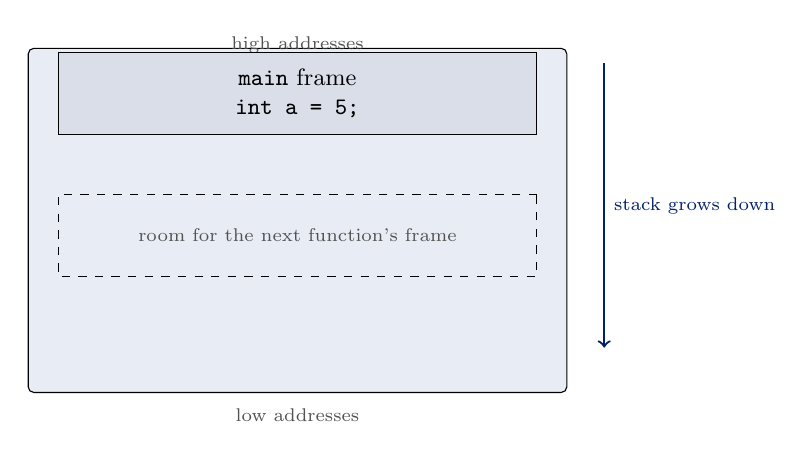
\begin{tikzpicture}[scale=0.95, every node/.style={scale=0.95}]
    \node[draw, fill=light-bg, minimum width=7.2cm, minimum height=4.6cm,
          rounded corners=2pt] at (0,-1.5) {};
    \node[font=\scriptsize, text=neutral] at (0,0.85) {high addresses};
    \node[draw, fill=primary-blue!15, minimum width=6.4cm, minimum height=1.1cm,
          align=center, font=\small] at (0,0.2)
          {\texttt{main} frame\\ \texttt{int a = 5;}};
    \node[draw, dashed, minimum width=6.4cm, minimum height=1.1cm,
          align=center, font=\scriptsize, text=neutral] at (0,-1.7)
          {room for the next function's frame};
    \draw[->, thick, color=primary-blue] (4.1,0.6) -- (4.1,-3.2)
      node[midway, right, font=\scriptsize] {stack grows down};
    \node[font=\scriptsize, text=neutral] at (0,-4.1) {low addresses};
  \end{tikzpicture}
  \caption{Stack growth, Step 1: \texttt{main} starts and its frame is created,
  holding \texttt{int a = 5;}. The stack grows \emph{downward} --- toward lower
  addresses.}
  \label{fig:stack1}
\end{figure}

\begin{example}[Stack growth, Step 2: \texttt{add} is called]
The call \texttt{add(x=5, y=3)} pushes a \emph{second} frame just below
\texttt{main}'s, holding the parameters (\texttt{x}, \texttt{y}) and the local
\texttt{int s = x + y;} --- which evaluates to \texttt{8}
(Figure~\ref{fig:stack2}). Every new function call pushes a new frame just below
the current one, so each new frame sits at a \key{lower} address than the frame
above it.
\end{example}

\begin{figure}[h]
  \centering
  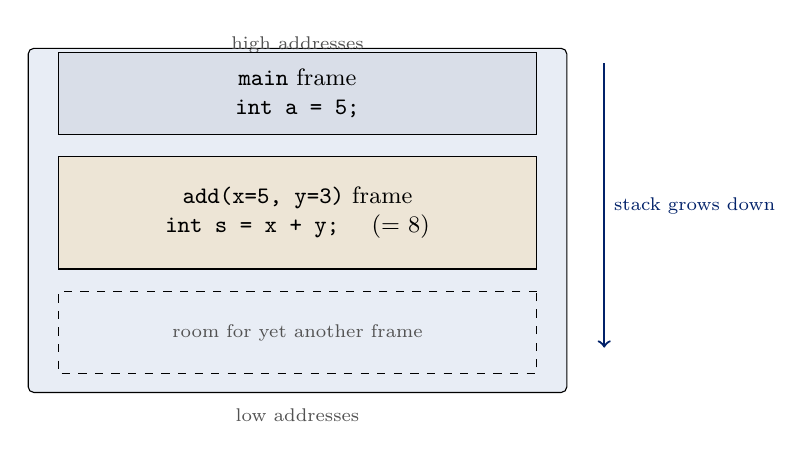
\begin{tikzpicture}[scale=0.95, every node/.style={scale=0.95}]
    \node[draw, fill=light-bg, minimum width=7.2cm, minimum height=4.6cm,
          rounded corners=2pt] at (0,-1.5) {};
    \node[font=\scriptsize, text=neutral] at (0,0.85) {high addresses};
    \node[draw, fill=primary-blue!15, minimum width=6.4cm, minimum height=1.1cm,
          align=center, font=\small] at (0,0.2)
          {\texttt{main} frame\\ \texttt{int a = 5;}};
    \node[draw, fill=primary-gold!25, minimum width=6.4cm, minimum height=1.5cm,
          align=center, font=\small] at (0,-1.4)
          {\texttt{add(x=5, y=3)} frame\\ \texttt{int s = x + y;} \quad (= 8)};
    \node[draw, dashed, minimum width=6.4cm, minimum height=1.1cm,
          align=center, font=\scriptsize, text=neutral] at (0,-3.0)
          {room for yet another frame};
    \draw[->, thick, color=primary-blue] (4.1,0.6) -- (4.1,-3.2)
      node[midway, right, font=\scriptsize] {stack grows down};
    \node[font=\scriptsize, text=neutral] at (0,-4.1) {low addresses};
  \end{tikzpicture}
  \caption{Stack growth, Step 2: the call to \texttt{add} pushes a second frame
  (parameters \texttt{x},\texttt{y} and local \texttt{s}) at a lower address than
  \texttt{main}'s frame.}
  \label{fig:stack2}
\end{figure}

\begin{example}[Stack growth, Step 3: \texttt{add} returns]
When \texttt{add} returns, its frame is popped off the stack --- it no longer
exists, and its memory is available again for the next call
(Figure~\ref{fig:stack3}). The answer \texttt{8} is copied back into
\texttt{main}'s frame as \texttt{int s = 8;}. The stack has returned to its
Step~1 shape.
\end{example}

\begin{figure}[h]
  \centering
  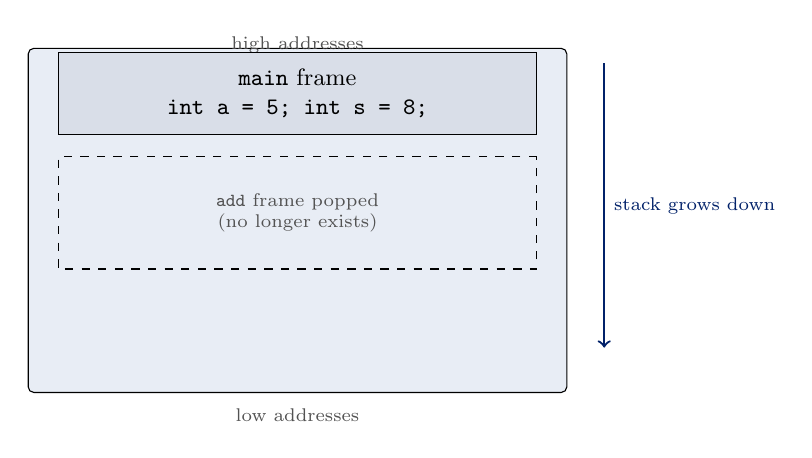
\begin{tikzpicture}[scale=0.95, every node/.style={scale=0.95}]
    \node[draw, fill=light-bg, minimum width=7.2cm, minimum height=4.6cm,
          rounded corners=2pt] at (0,-1.5) {};
    \node[font=\scriptsize, text=neutral] at (0,0.85) {high addresses};
    \node[draw, fill=primary-blue!15, minimum width=6.4cm, minimum height=1.1cm,
          align=center, font=\small] at (0,0.2)
          {\texttt{main} frame\\ \texttt{int a = 5; int s = 8;}};
    \node[draw, dashed, minimum width=6.4cm, minimum height=1.5cm,
          align=center, font=\scriptsize, text=neutral] at (0,-1.4)
          {\texttt{add} frame popped\\ (no longer exists)};
    \draw[->, thick, color=primary-blue] (4.1,0.6) -- (4.1,-3.2)
      node[midway, right, font=\scriptsize] {stack grows down};
    \node[font=\scriptsize, text=neutral] at (0,-4.1) {low addresses};
  \end{tikzpicture}
  \caption{Stack growth, Step 3: \texttt{add} returns, its frame is popped and
  its memory is free again; \texttt{8} was copied back into \texttt{main}'s
  frame.}
  \label{fig:stack3}
\end{figure}

The three steps together are the whole story of automatic storage: lifetime is
decided by the compiler, not by you. A local variable lives exactly as long as
its enclosing call. This is precisely why returning a pointer to a local
variable is a bug --- the frame it pointed into ceases to exist the instant the
function returns.

\subsection{Why the stack is not enough}

Consider a requirement the stack simply cannot meet: the user enters the number
of records only after the program starts, and we may need space for 3 records
today and 300 tomorrow. The stack decides every frame's size at compile time and
discards every local when its call returns. So the stack fails on both counts:
we do not know the size in advance, and we may want the records to remain after
the helper function that created them returns.

What we need is storage whose size is decided at run time and
whose lifetime \emph{we} control rather than the compiler. That is exactly what
the \key{heap} provides, and the only way to reach the heap is through a
pointer. Wirth puts the underlying argument crisply: recursive (variable-sized)
structures ``cannot be assigned a fixed amount of storage,'' so the compiler
cannot associate specific addresses with them; the resolution is \emph{dynamic
allocation} --- allocating store to components when they come into existence
during program execution --- with fixed storage reserved only for the
\emph{address} of the component \cite{Wirth2004_algorithms_data_structures}
(p.~111).

\begin{example}[A prediction worth making before the vocabulary]
Two declarations:
\begin{itemize}
  \item \texttt{int score = 80;}
  \item \texttt{int *p = malloc(sizeof(int));}
\end{itemize}
Which variable can outlive the function that created it? The local variable
\texttt{score} belongs to its function call and dies with it. The heap block ---
the one requested by \texttt{malloc} --- remains until the program releases it
with \texttt{free}. The pointer \texttt{p} is only the \emph{handle}; the block
is the data storage. Answer: the \emph{block}, not the variable that names it.
The exact call that makes this happen (\texttt{malloc} and \texttt{sizeof}) comes
in Section~\ref{sec:heap}.
\end{example}

\section{Pointers: The Handle on Memory}

\textbf{Read alongside:} Wirth, \S4.2, p.111 --- the dynamic-allocation argument and the address-as-handle picture.

\begin{definitionbox}{Pointer}
A variable that stores an address. Its type records what kind of object resides
at that address.
\end{definitionbox}

An ordinary variable stores a value such as \texttt{80}. A pointer stores a
\emph{place} such as ``where the score lives.'' The type tells C what kind of
value is at that place. The declaration \texttt{int *p;} means: \texttt{p} can
point to an \texttt{int} \cite{Wirth2004_algorithms_data_structures}.

Figure~\ref{fig:pointer-picture} draws the distinction. The variable \texttt{p}
on the left does not contain the score itself --- it contains an address. The box
on the right holds the actual value \texttt{80}. The arrow labelled ``points
to'' is the whole idea: \texttt{p} tells us where the score can be found.

\begin{figure}[h]
  \centering
  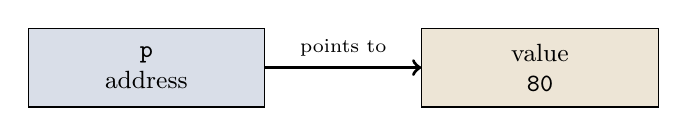
\begin{tikzpicture}[every node/.style={font=\small}]
    \node[draw, fill=primary-blue!15, minimum width=3.0cm, minimum height=1cm,
      align=center]
      (p) at (-2.5,0) {\texttt{p}\\address};
    \node[draw, fill=primary-gold!25, minimum width=3.0cm, minimum height=1cm,
      align=center]
      (x) at (2.5,0) {value\\\texttt{80}};
    \draw[->, very thick] (p.east) -- (x.west)
      node[midway, above, font=\scriptsize] {points to};
  \end{tikzpicture}
  \caption{A pointer picture: \texttt{p} holds an address; the value \texttt{80}
  lives at that address. The pointer is the handle, not the data.}
  \label{fig:pointer-picture}
\end{figure}

\subsection{Pointers reach structures}

Pointers earn their keep when they point at \emph{structures}. The basic
building block for most of this course is a two-field node:

\begin{center}
\small
\begin{verbatim}
struct node {
  int data;
  struct node *next;
};
\end{verbatim}
\end{center}

The \texttt{data} field stores the value; the \texttt{next} field stores the
address of \emph{another} node. If there is no next node, set
\texttt{next = NULL}. This is the seed of a linked list, studied properly in
Week 6; here it appears only so that we can point at something real.
\muted{The list handle will be called \texttt{head} starting Week 6; here the
node is just \texttt{p}.} For the
field-access we prefer the arrow form: writing \texttt{p->data} reads the
\texttt{data} field of the node \texttt{p} points at, and \texttt{p->next} reads
its successor link. (The equivalent \texttt{(*p).data} is correct C but noisier;
this course uses \texttt{->} throughout.)

\subsection{The safe empty pointer}

\begin{definitionbox}{\texttt{NULL}}
The address value meaning ``points at nothing.'' A pointer set to \texttt{NULL}
is currently empty; reading through it is undefined behaviour --- in practice, a
crash.
\end{definitionbox}

\texttt{NULL} is the agreed way to show that a pointer is not pointing to a
valid object. Use it to mark empty state, check a pointer before using the
object it should point to, and never read through an empty pointer. The
canonical example of its meaning: \texttt{struct node *p = NULL;} says ``this
pointer reaches nothing yet.'' One notation convention holds for the whole
term: the null pointer is always written \texttt{NULL} in uppercase, and the
list handle is always named \texttt{head} starting Week 6.

\section{One Heap Block}
\label{sec:heap}

\textbf{Read alongside:} Wirth, \S4.2, p.111 (dynamic allocation); Horowitz \& Sahni, Ch.~1 (chapter-level).

This section does one thing repeatedly: allocate a block on the heap, use it,
and return it. The whole memory-discipline of the course is these three
moves, and the section works through C's whole heap-allocation interface ---
\texttt{malloc}, \texttt{sizeof}, \texttt{calloc}, \texttt{realloc}, and
\texttt{free} --- in the order a program actually needs them.

\subsection{Requesting memory: \texttt{malloc} and \texttt{sizeof}}

The call \texttt{malloc(n)} asks the heap for \texttt{n} \emph{bytes} of memory
and returns their address, or \texttt{NULL} if the request cannot be met. You
should never count those bytes by hand; the \texttt{sizeof} operator computes
them for you and stays correct when the type or the target machine changes.
\texttt{malloc} itself never knows how big, say, an \texttt{int} is on its
own --- \texttt{sizeof} is what tells it, and every allocation request in this
course uses it: \texttt{sizeof(int)} is typically \texttt{4}, and
\texttt{sizeof(struct node)} is the size of the \texttt{data} field plus the
\texttt{next} field together.

\begin{example}[The basic pattern: one integer on the heap]
{\footnotesize
\begin{verbatim}
int *p = malloc(sizeof(int));
if (p == NULL) return 1;
*p = 80;
\end{verbatim}
}
Reading it line by line:
\begin{enumerate}
  \item \texttt{malloc(sizeof(int))} requests from the heap exactly as many
    bytes as one \texttt{int} needs, and returns their address.
  \item \texttt{p} stores that address. If the request failed, \texttt{malloc}
    returns \texttt{NULL}; the \texttt{if} guard converts that failure into a
    controlled exit instead of a crash later.
  \item \texttt{*p = 80;} writes the value \texttt{80} into the heap block ---
    the block \emph{at} the address \texttt{p} holds. (Note the difference from
    the pointer picture in Figure~\ref{fig:pointer-picture}: there \texttt{p}
    pointed at a pre-existing box; here the box did not exist until this call.)
\end{enumerate}
The name \texttt{p} is not the heap block; the block is at the address
\texttt{p} contains.
\end{example}

\subsection{Zero-initialized memory: \texttt{calloc}}

\begin{definitionbox}{\texttt{calloc}}
\texttt{calloc(n, size)} allocates space for \texttt{n} items of \texttt{size}
bytes each, and sets \emph{every byte} of that space to \texttt{0}.
\end{definitionbox}

{\footnotesize
\begin{verbatim}
int *counts = calloc(5, sizeof(int));
if (counts == NULL) return 1;
\end{verbatim}
}
The declaration above requests room for five integers, exactly as
\texttt{malloc(5 * sizeof(int))} would, but with one added guarantee:
\key{\texttt{calloc} zero-initializes; \texttt{malloc} does not.} That
guarantee is the entire difference between the two calls --- same style of
request, same \texttt{NULL} check, different starting content.

\begin{example}[\texttt{malloc} vs.\ \texttt{calloc}: what is actually in the block]
Figure~\ref{fig:malloc-calloc} draws two independent four-byte requests side
by side. On the left, \texttt{malloc(4 * sizeof(int))} hands back four bytes
whose content is \key{unspecified} --- drawn as \texttt{?} because the memory
could contain anything left over from a previous use of that space; reading
those bytes \emph{before writing them} is undefined behaviour. On the right,
\texttt{calloc(4, sizeof(int))} hands back four bytes already \key{set to
zero}; a program may read them immediately, before ever writing to them, and
the value it gets back is well-defined: \texttt{0}. The two calls request the
same amount of memory; only the starting content differs, and only
\texttt{calloc} pays the (small) extra cost of writing zeros before handing
the block back.
\end{example}

\begin{figure}[h]
  \centering
  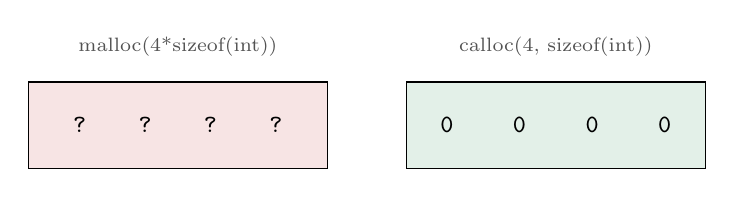
\begin{tikzpicture}[every node/.style={font=\small}]
    \node[font=\scriptsize, text=neutral] at (-2.4,1.0) {malloc(4*sizeof(int))};
    \node[draw, fill=negative!12, minimum width=3.8cm, minimum height=1.1cm,
      align=center, font=\ttfamily\small]
      (m) at (-2.4,0) {? \quad ? \quad ? \quad ?};
    \node[font=\scriptsize, text=neutral] at (2.4,1.0) {calloc(4, sizeof(int))};
    \node[draw, fill=positive!12, minimum width=3.8cm, minimum height=1.1cm,
      align=center, font=\ttfamily\small]
      (c) at (2.4,0) {0 \quad\; 0 \quad\; 0 \quad\; 0};
  \end{tikzpicture}
  \caption{\texttt{malloc} vs.\ \texttt{calloc}: \texttt{malloc} hands back
  four unspecified bytes (reading before writing is undefined behaviour);
  \texttt{calloc} hands back four bytes already zeroed.}
  \label{fig:malloc-calloc}
\end{figure}

\subsection{Resizing a block: \texttt{realloc}}

\begin{definitionbox}{\texttt{realloc}}
\texttt{realloc(p, newsize)} resizes the block \texttt{p} points to,
preserving its existing content up to the smaller of the old and new sizes.
The block \key{may move} --- always keep the returned pointer.
\end{definitionbox}

{\footnotesize
\begin{verbatim}
int *bigger = realloc(p, 10 * sizeof(int));
if (bigger == NULL) return 1;  // p is still valid here
p = bigger;
\end{verbatim}
}
Two details in this idiom matter more than they look. First, the check is
against \texttt{bigger}, not against \texttt{p} --- if \texttt{realloc} fails,
it returns \texttt{NULL} but leaves the \emph{original} block at \texttt{p}
untouched, so overwriting \texttt{p} with a possibly-\texttt{NULL} result
before checking would silently lose access to still-valid memory. Second,
\texttt{p} is only reassigned to \texttt{bigger} \emph{after} the check
succeeds.

\begin{example}[Growing an array with \texttt{realloc}]
Start with \texttt{p = malloc(3 * sizeof(int))} holding \texttt{10 20 30}.
Trace what happens, one statement at a time, when the array needs to grow to
five slots:
\begin{enumerate}
  \item \texttt{p = realloc(p, 5 * sizeof(int));} --- the request asks for a
    block of five integers' worth of space, built from the existing block at
    \texttt{p}.
  \item The first three ints (\texttt{10}, \texttt{20}, \texttt{30}) are
    \key{copied} into the new block, in the same order, by \texttt{realloc}
    itself --- the caller does not write this copy.
  \item The two new slots (index 3 and index 4) are \key{unspecified} ---
    \texttt{realloc} does not zero new space; only \texttt{calloc} zeros
    space. A program that needs the new slots to start at zero must set them
    explicitly after the call.
\end{enumerate}
\muted{If \texttt{realloc} returns \texttt{NULL}, the original block at
\texttt{p} is untouched and still valid --- never overwrite \texttt{p} with
the raw result before checking it, exactly as in the idiom above.}
\end{example}

\subsection{Allocate a complete node: the safer engineering pattern}

\begin{example}[Allocate a complete node: the safer engineering pattern]
{\footnotesize
\begin{verbatim}
struct node *p =
    malloc(sizeof(struct node));
if (p == NULL) return 1;
p->data = 42;
p->next = NULL;
\end{verbatim}
}
This is the pattern the course will reuse every week:
\begin{enumerate}
  \item \texttt{sizeof(struct node)} asks for exactly one node's bytes --- not a
    hand-counted \texttt{8} or \texttt{12}, which would be wrong the moment a
    field is added or the code is recompiled for another machine.
  \item The result is checked against \texttt{NULL} before anything touches the
    block.
  \item \texttt{p->data = 42;} stores a value in the node's \texttt{data} field.
  \item \texttt{p->next = NULL;} makes the node's \emph{end} explicit. The node
    has a clear stop: the next link is empty.
\end{enumerate}
Initialising every field makes the node's state predictable; an uninitialised
field would contain garbage.
\end{example}

\subsection{Audit the node before you ship it}

A small program is not finished when it compiles. The deck supplies a four-point
review checklist that doubles as this course's allocation invariant, and it is
worth internalising as a habit:

\begin{enumerate}
  \item Was the allocation checked against \texttt{NULL}?
  \item Was every field initialised before the node was used?
  \item Is there exactly one clear owner responsible for \texttt{free(p)}?
  \item Can the program reach the node later, or has its pointer been lost?
\end{enumerate}

The engineering habit behind the list: test both the normal path and the
allocation-failure path. In C, out-of-memory is not an exception the runtime
raises for you; it is a \texttt{NULL} return you must notice.

\subsection{Trace it before running it}

Reading C and running C are different skills. Before running the two lines

{\footnotesize
\begin{verbatim}
int *p = malloc(sizeof(int));
*p = 80;
\end{verbatim}
}

the deck asks: \emph{after these lines, what is true?} Answer, state by state:

\begin{enumerate}
  \item \texttt{p} contains an address --- the address \texttt{malloc} returned.
  \item The heap block at that address contains \texttt{80} --- written there by
    \texttt{*p = 80;}.
  \item The name \texttt{p} itself is \emph{not} the heap block. They are two
    different objects in two different regions (Figure~\ref{fig:happened}).
\end{enumerate}

The challenge in the same frame: \emph{which line would fail if
\texttt{p == NULL}?} Line two. Dereferencing \texttt{NULL} with \texttt{*p} is
undefined behaviour --- in practice a crash. Line one would have already told you
the allocation failed, if you had checked.

\begin{figure}[h]
  \centering
  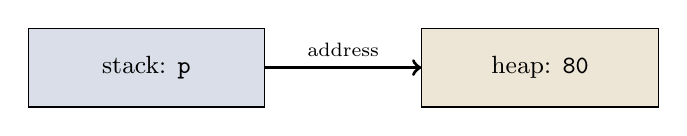
\begin{tikzpicture}[every node/.style={font=\small}]
    \node[draw, fill=primary-blue!15, minimum width=3cm, minimum height=1cm]
      (p) at (-2.5,0) {stack: \texttt{p}};
    \node[draw, fill=primary-gold!25, minimum width=3cm, minimum height=1cm]
      (box) at (2.5,0) {heap: \texttt{80}};
    \draw[->, very thick] (p.east) -- (box.west)
      node[midway, above, font=\scriptsize] {address};
  \end{tikzpicture}
  \caption{What happened after the two lines: \texttt{p} lives on the stack and
  holds the address of a heap block containing \texttt{80}. The pointer and the
  block are separate objects in separate regions.}
  \label{fig:happened}
\end{figure}

\subsection{How the heap grows}

Just as the stack picture was built from three steps, the heap gets the same
treatment. The growing arrow runs \emph{upward}: the heap grows toward higher
addresses, opposite to the stack.

\begin{example}[Heap growth, Step 1: one \texttt{malloc} for three integers]
One \texttt{malloc} request with room for three integers grew the used heap
upward, placing a block that holds \texttt{10}, \texttt{20}, \texttt{30}
(Figure~\ref{fig:heap1}). The block survives after the allocating function
returns --- that is the heap's whole point.
\end{example}

\begin{figure}[h]
  \centering
  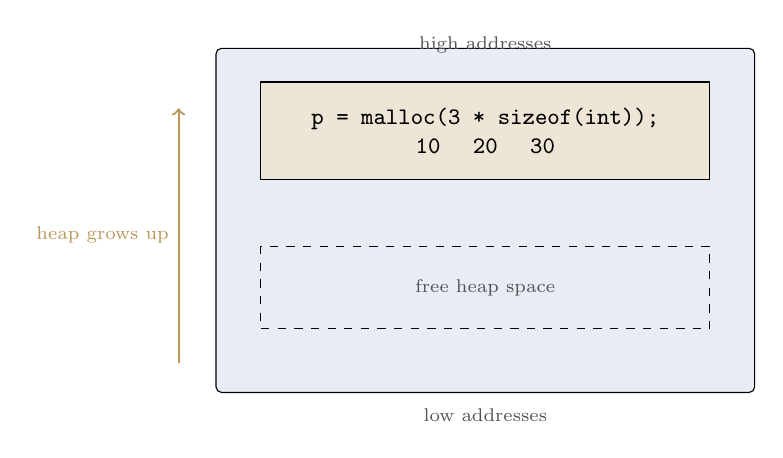
\begin{tikzpicture}[scale=0.95, every node/.style={scale=0.95}]
    \node[draw, fill=light-bg, minimum width=7.2cm, minimum height=4.6cm,
          rounded corners=2pt] at (0,-1.5) {};
    \node[font=\scriptsize, text=neutral] at (0,0.85) {high addresses};
    \node[draw, fill=primary-gold!25, minimum width=6.0cm, minimum height=1.3cm,
          align=center, font=\small] at (0,-0.3)
          {\texttt{p = malloc(3 * sizeof(int));}\\ \texttt{10} \quad \texttt{20} \quad \texttt{30}};
    \node[draw, dashed, minimum width=6.0cm, minimum height=1.1cm,
          align=center, font=\scriptsize, text=neutral] at (0,-2.4)
          {free heap space};
    \draw[->, thick, color=primary-gold] (-4.1,-3.4) -- (-4.1,0.0)
      node[midway, left, font=\scriptsize] {heap grows up};
    \node[font=\scriptsize, text=neutral] at (0,-4.1) {low addresses};
  \end{tikzpicture}
  \caption{Heap growth, Step 1: \texttt{malloc(3 * sizeof(int))} places one
  block holding \texttt{10}, \texttt{20}, \texttt{30}; the used heap grew
  upward.}
  \label{fig:heap1}
\end{figure}

\begin{example}[Heap growth, Step 2: a second block]
The second request places \texttt{q}'s block at a \key{higher} address than
\texttt{p}'s (Figure~\ref{fig:heap2}). Blocks are independent: each keeps its
own data, and one block's values cannot reach into the other's.
\end{example}

\begin{figure}[h]
  \centering
  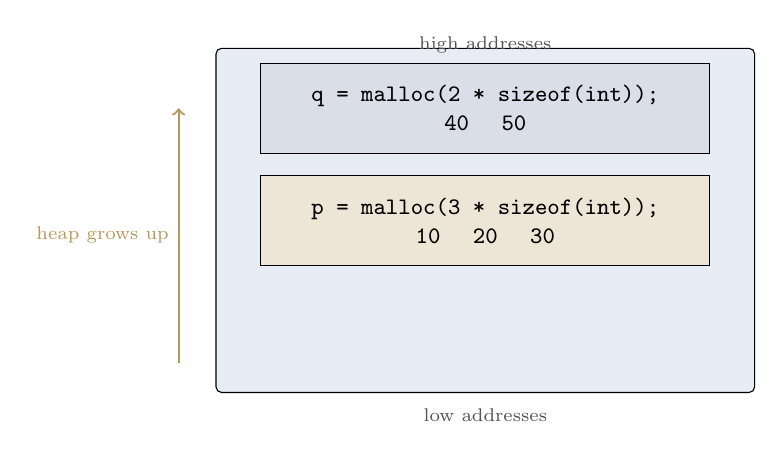
\begin{tikzpicture}[scale=0.95, every node/.style={scale=0.95}]
    \node[draw, fill=light-bg, minimum width=7.2cm, minimum height=4.6cm,
          rounded corners=2pt] at (0,-1.5) {};
    \node[font=\scriptsize, text=neutral] at (0,0.85) {high addresses};
    \node[draw, fill=primary-gold!25, minimum width=6.0cm, minimum height=1.2cm,
          align=center, font=\small] at (0,-1.5)
          {\texttt{p = malloc(3 * sizeof(int));}\\ \texttt{10} \quad \texttt{20} \quad \texttt{30}};
    \node[draw, fill=primary-blue!15, minimum width=6.0cm, minimum height=1.2cm,
          align=center, font=\small] at (0,0.0)
          {\texttt{q = malloc(2 * sizeof(int));}\\ \texttt{40} \quad \texttt{50}};
    \draw[->, thick, color=primary-gold] (-4.1,-3.4) -- (-4.1,0.0)
      node[midway, left, font=\scriptsize] {heap grows up};
    \node[font=\scriptsize, text=neutral] at (0,-4.1) {low addresses};
  \end{tikzpicture}
  \caption{Heap growth, Step 2: a second \texttt{malloc} places \texttt{q}'s
  block at a higher address; the two blocks are independent.}
  \label{fig:heap2}
\end{figure}

\begin{example}[Heap growth, Step 3: \texttt{free} returns a block]
{\footnotesize
\begin{verbatim}
free(p);
p = NULL;
\end{verbatim}
}
\texttt{free(p)} gives \texttt{p}'s block back to the system --- it is no longer
usable --- and the used heap can shrink again (Figure~\ref{fig:heap3}).
\texttt{q}'s block is untouched. Setting \texttt{p} to \texttt{NULL} afterwards
makes the old pointer visibly empty, so it can never be mistaken for a live
handle.
\end{example}

\begin{figure}[h]
  \centering
  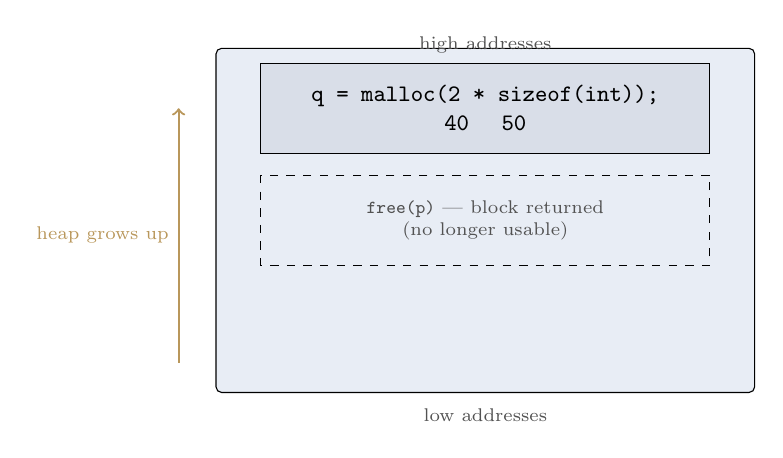
\begin{tikzpicture}[scale=0.95, every node/.style={scale=0.95}]
    \node[draw, fill=light-bg, minimum width=7.2cm, minimum height=4.6cm,
          rounded corners=2pt] at (0,-1.5) {};
    \node[font=\scriptsize, text=neutral] at (0,0.85) {high addresses};
    \node[draw, dashed, minimum width=6.0cm, minimum height=1.2cm,
          align=center, font=\scriptsize, text=neutral] at (0,-1.5)
          {\texttt{free(p)} --- block returned\\ (no longer usable)};
    \node[draw, fill=primary-blue!15, minimum width=6.0cm, minimum height=1.2cm,
          align=center, font=\small] at (0,0.0)
          {\texttt{q = malloc(2 * sizeof(int));}\\ \texttt{40} \quad \texttt{50}};
    \draw[->, thick, color=primary-gold] (-4.1,-3.4) -- (-4.1,0.0)
      node[midway, left, font=\scriptsize] {heap grows up};
    \node[font=\scriptsize, text=neutral] at (0,-4.1) {low addresses};
  \end{tikzpicture}
  \caption{Heap growth, Step 3: \texttt{free(p)} returns \texttt{p}'s block to
  the system; \texttt{q}'s block is untouched.}
  \label{fig:heap3}
\end{figure}

\subsection{Returning the memory}

\texttt{free} is the counterpart of \texttt{malloc}, \texttt{calloc}, and
\texttt{realloc} alike: every block obtained from any of the three needs a
matching \texttt{free}. The recommended sequence is two lines that travel
together:

{\footnotesize
\begin{verbatim}
free(p);
p = NULL;
\end{verbatim}
}

The first line returns the heap block to the system. The second makes the old
pointer visibly empty, so the handle cannot accidentally be used as though the
block still existed. \good{Request memory, use it, return it.} This three-word
rule is the entire memory-discipline of the course, and the two failures that
violate it are the two beginner mistakes.

\subsection{Two beginner mistakes}

\begin{itemize}
  \item \bad{Memory leak}: forget to call \texttt{free}; the block stays
    reserved for the whole program, and if the pointer is overwritten without
    freeing, nothing can ever reach the block again. Nothing crashes --- the
    program simply grows until it dies.
  \item \bad{Dangling pointer}: use a pointer after its block was freed. The
    block is gone (or reused), so reads return garbage and writes corrupt
    whatever now occupies that space.
\end{itemize}

The simple habit that prevents both: \key{keep track of who requested the
memory and who will return it}. Decide the single owner at the moment of
allocation, and that owner is responsible for exactly one \texttt{free}.

\section{Simple Contracts}

\textbf{Read alongside:} Sedgewick \& Wayne, \textit{Algorithms}, \S1.2, p.64 --- the data-type/ADT definition; \S1.3, p.120 --- bag as a collection type; Karumanchi, \textit{Data Structures and Algorithms Made Easy}, \S1.4, p.18 (PDF) --- the two-part ADT definition and the commonly-used-ADTs list; Aho, Hopcroft \& Ullman, Ch.~1 (chapter-level).

We can now build a structure and reach it through a pointer. The remaining
difficulty is describing one without drowning in pointers --- which brings us to
the course's central abstraction.

\begin{definitionbox}{Abstract data type (ADT)}
A description of what we can do with data, without saying how it is stored: a
promise about operations.
\end{definitionbox}

Sedgewick \& Wayne put it as cleanly as anyone: a data type is ``a set of values
and a set of operations on those values'' \cite{Sedgewick2011_algorithms}
(p.~64), and the \emph{abstract} data type is that contract stated before any
implementation decides how it is met. An ADT is a promise about operations; the
implementation is the code and memory arrangement behind the promise; and
different implementations can follow the same promise.

Karumanchi's treatment makes the same contract concrete by splitting it into
two named parts: an ADT ``consists of two parts: 1. Declaration of data[;]
2. Declaration of operations'' \cite{Karumanchi2017_data_structures_algorithms_made_easy}
(p.~18, PDF). \muted{The two textbook framings agree: Sedgewick's ``set of
values and set of operations'' is exactly Karumanchi's ``declaration of data''
and ``declaration of operations.''}

\begin{example}[A very small bag]
The deck's running example is a \key{bag of integers} --- one of Sedgewick \&
Wayne's three collection types (p.~120) \cite{Sedgewick2011_algorithms} ---
supporting exactly three operations:
\begin{enumerate}
  \item \texttt{insert(x)} --- put \texttt{x} into the bag.
  \item \texttt{member(x)} --- answer whether \texttt{x} is present.
  \item \texttt{size()} --- report how many items are present.
\end{enumerate}
The contract does not yet say whether the bag uses an array or a list. That is
the point: the contract deliberately withholds the implementation.
\end{example}

\subsection{One contract, two possible implementations}

Both a dynamic array and a chain of linked nodes can honour the bag contract.
Figure~\ref{fig:adt} draws the relationship: the contract box on top, two
implementation boxes below, connected by plain arrows.

\begin{figure}[h]
  \centering
  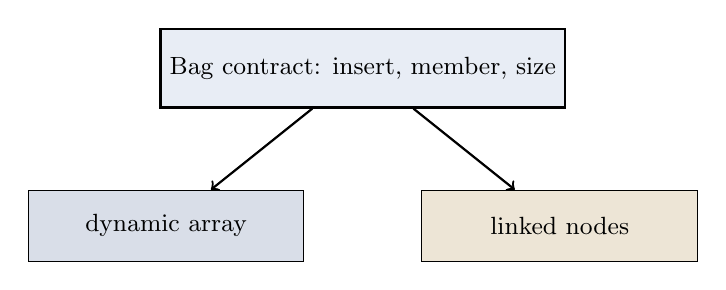
\begin{tikzpicture}[every node/.style={font=\small}]
    \node[draw, thick, fill=light-bg, minimum width=5cm, minimum height=1cm]
      (adt) at (0,2) {Bag contract: insert, member, size};
    \node[draw, fill=primary-blue!15, minimum width=3.5cm, minimum height=0.9cm]
      (array) at (-2.5,0) {dynamic array};
    \node[draw, fill=primary-gold!25, minimum width=3.5cm, minimum height=0.9cm]
      (list) at (2.5,0) {linked nodes};
    \draw[->, thick] (adt) -- (array);
    \draw[->, thick] (adt) -- (list);
  \end{tikzpicture}
  \caption{One contract, two implementations. Same operations, different
  internal arrangement. The caller's code does not change when the bottom box
  does --- that substitutability is the value of the abstraction.}
  \label{fig:adt}
\end{figure}

The key distinction, stated once and reused all term: \key{same operations,
different internal arrangement}. This framing runs the whole course. Weeks 3
and 7 both implement a \key{stack}, once over an array and once over a chain of
nodes. Weeks 5 and 7 do the same for a \key{queue}. Week 6 and Week 10 both
implement a \key{lookup table} for the identifiers in our expression processor,
first as a list and then as a hash table. Every time, the code that \emph{uses}
the structure is written against the contract and does not care which
implementation it received.

\subsection{This course is a tour of ADTs}

The bag is a warm-up, not a one-off example: Linked Lists, Stacks, Queues,
Priority Queues, Binary Trees, Hash Tables, and Graphs are all
commonly used ADTs \cite{Karumanchi2017_data_structures_algorithms_made_easy}
(p.~18, PDF), and Weeks 3 through 12 work through this list one ADT at a time.
Each week repeats the same three-beat shape --- \emph{state the question}
(``What is a Stack?''), \emph{state the contract} (``Stack ADT''), \emph{then
implement it} (``Implementation'') --- in that order, every time. \muted{Watch
for this shape across the term: the contract is always stated and argued for
before a single line of implementation is written.}

\begin{example}[Classifying contract statements vs.\ implementation statements]
Is each statement part of the contract, or part of one implementation?
\begin{enumerate}
  \item ``\texttt{member(7)} answers yes or no.'' --- \good{contract}. It
    describes what a user can ask.
  \item ``The values are stored in an array.'' --- \bad{implementation}. It
    describes \emph{how} one particular bag is built.
  \item ``\texttt{size()} reports the number of values.'' --- \good{contract}.
    It describes what a user can ask.
\end{enumerate}
The first and third describe what users can ask; the second describes how. This
two-way split --- what vs.\ how --- is the habit to build now: \key{state the
contract before writing a line of the implementation}.
\end{example}

\section{What We Cannot Yet Answer}

We can now build two implementations of the same ADT, and we have no vocabulary
whatever for saying which is better --- only ``it felt faster,'' which is not an
argument.

Week 2 supplies that vocabulary. \key{Algorithm analysis} counts an algorithm's
basic operations as a function of the input size $n$, giving an exact cost
function $T(n)$, then compresses that count into an asymptotic class ---
$O$, $\Omega$, $\Theta$ --- and separates the \emph{best}, \emph{worst}, and
\emph{average} case, so that two implementations can be compared without ever
running either of them. The bag's two implementations differ \emph{only} in
cost; Week 2 is how we say that precisely.

\subsection*{Exercises}

\begin{enumerate}
  \item Rewrite \texttt{larger} from Section~\ref{sec:structured} so that it
    prints the largest of \emph{three} exam marks instead of two, and identify
    which of the three control patterns (sequence, selection, iteration) your
    new version needs that the original did not.
  \item If \texttt{p} lives on the stack and the node lives on the heap, what
    exactly is lost when \texttt{main} returns without calling \texttt{free}?
    Who could still reach that node?
  \item Draw the complete picture for these four lines, then state what is true
    after each one:
{\footnotesize
\begin{verbatim}
struct node *p = malloc(sizeof(struct node));
if (p == NULL) return 1;
p->data = 7;
p->next = NULL;
\end{verbatim}
}
    Your drawing should show which region each object lives in and the value of
    every field.
  \item In the heap-growth trace, the second block (\texttt{q}) sits at a
    \emph{higher} address than the first (\texttt{p}). If you now call
    \texttt{free(q)} and then \texttt{malloc} a block of three integers, what
    can you say about where the new block lands? (Hint: think about what
    ``free space'' the heap reuses, not about exact addresses.)
  \item Suppose \texttt{p = calloc(3, sizeof(int));} and later
    \texttt{q = realloc(p, 6 * sizeof(int));} succeeds. After these two lines,
    what values are in slots 0--2 of the block \texttt{q} points to, and what
    can you say about slots 3--5? Justify each answer from the definitions of
    \texttt{calloc} and \texttt{realloc} given in Section~\ref{sec:heap}.
\end{enumerate}

\subsection*{Solutions}

\begingroup\small
\begin{enumerate}
  \item \textbf{Three marks, one new pattern:} a three-argument version, e.g.
{\footnotesize
\begin{verbatim}
int largest3(int a, int b, int c) {
  int m = a;                 // sequence
  if (b > m) m = b;          // selection
  if (c > m) m = c;          // selection
  return m;
}
\end{verbatim}
}
    still needs no loop, because the count of marks (three) is fixed and known
    at compile time --- two \texttt{if} statements suffice, so no new pattern
    is required. \emph{Iteration} only becomes necessary once the number of
    marks is not fixed in the source code, e.g. reading marks from an array of
    unknown length and comparing each one in turn; that version would need a
    \texttt{for} loop over the array, which is exactly the boundary the deck's
    original frame points at: ``a loop appears the moment we compare more than
    two marks'' in the general case of an arbitrary count.
  \item \textbf{What is lost:} the \emph{reach}. \texttt{main}'s frame (which
    held \texttt{p}, the only pointer to the node) is popped when
    \texttt{main} returns, so the node's address disappears. The node itself is
    still allocated on the heap --- it has not been freed --- but no live
    pointer names it any more. Nobody can reach that node; it is a memory leak.
    The block stays reserved for the rest of the program's life.
  \item \textbf{The complete picture:}
    \begin{itemize}
      \item After line 1: \texttt{p} (on the stack) holds an address returned by
        \texttt{malloc}; a one-node block now exists on the heap, with garbage
        in both fields because nothing has written to it yet.
      \item After line 2 (assuming the check passed): the address is known to be
        valid; execution continues.
      \item After line 3: the heap node's \texttt{data} field holds \texttt{7}.
      \item After line 4: the heap node's \texttt{next} field holds
        \texttt{NULL}, marking the end of the chain. The stack holds \texttt{p};
        the heap holds a node with \texttt{data = 7}, \texttt{next = NULL}.
    \end{itemize}
  \item \textbf{The new block's location:} freeing \texttt{q} returns its
    two-integer block to the heap's free space. A subsequent \texttt{malloc} of
    three integers will be served from \emph{available} free space; the exact
    address is the allocator's choice and not something the program may rely on.
    What you \emph{can} say is general: the allocator reuses freed space, so the
    heap's used region can shrink and later regrow --- the important invariant
    is that each block is reached only through a live pointer, never through a
    guess about its neighbour.
  \item \textbf{\texttt{calloc} then \texttt{realloc}:} \texttt{calloc(3, sizeof(int))}
    zero-initializes its whole block, so immediately after the first line
    slots 0--2 all hold \texttt{0}. \texttt{realloc(p, 6 * sizeof(int))}
    preserves the existing content up to the smaller of the old and new sizes
    --- the old size was three ints, so slots 0--2 are copied unchanged into
    the new block and remain \texttt{0}. But \texttt{realloc} is not
    \texttt{calloc}: it does \emph{not} zero the newly added space, so slots
    3--5 are \key{unspecified} --- the same ``garbage until written'' state
    \texttt{malloc} produces, not guaranteed zero. A program that needs slots
    3--5 to start at zero must set them explicitly after the \texttt{realloc}
    call, exactly as the \texttt{realloc} worked example in
    Section~\ref{sec:heap} notes for its own two new slots.
\end{enumerate}
\endgroup

\subsection*{Summary}

\begin{itemize}
  \item A program is \key{algorithms} plus \key{data structures}.
    \key{Structured programming} disciplines the first term: every program is
    built from exactly three control patterns --- sequence, selection,
    iteration --- decomposed top-down into named, reusable functions; that
    same discipline (name the contract, then implement it) is what this
    course applies to data.
  \item \key{Stack} storage is automatic and scope-bound: a frame is pushed on
    call and popped on return, and the stack grows \emph{down}. \key{Heap}
    storage is run-time sized and lifetime-controlled by you: it grows
    \emph{up}, and its lifetime is controlled by explicit allocation and
    release rather than by function scope.
  \item A \key{pointer} stores an address --- a handle on a value or structure,
    never the object itself. \texttt{NULL} means ``points to nothing,'' and
    dereferencing it is undefined behaviour.
  \item The allocation idiom: \texttt{malloc} with \texttt{sizeof} for
    unspecified content, \texttt{calloc} when the block must start
    zero-initialized, \texttt{realloc} to resize an existing block (the block
    may move --- always keep the returned pointer, and never overwrite the old
    pointer before checking the result), and \texttt{free} to return the
    block once it is no longer needed. Every request is checked against
    \texttt{NULL} before the block is used.
  \item The two silent failures: \bad{memory leak} (never freed) and
    \bad{dangling pointer} (used after being freed). Every allocation gets
    exactly one owner.
  \item An \key{ADT} is a contract about operations; a \key{data structure} is
    one implementation of it. State the contract before writing the code, and
    the rest of the course compares implementations of shared contracts.
  \item The rest of this course is a tour of ADTs --- Linked Lists, Stacks,
    Queues, Priority Queues, Binary Trees, Hash Tables, and
    Graphs --- each one: contract first, implementation second.
\end{itemize}

\bibliography{../../Bibliography_base}
\bibliographystyle{plain}

\end{document}
